\documentclass[11pt,a4paper,]{article}
\usepackage{lmodern}

\usepackage{amssymb,amsmath}
\usepackage{ifxetex,ifluatex}
\usepackage{fixltx2e} % provides \textsubscript
\ifnum 0\ifxetex 1\fi\ifluatex 1\fi=0 % if pdftex
  \usepackage[T1]{fontenc}
  \usepackage[utf8]{inputenc}
\else % if luatex or xelatex
  \usepackage{unicode-math}
  \defaultfontfeatures{Ligatures=TeX,Scale=MatchLowercase}
\fi
% use upquote if available, for straight quotes in verbatim environments
\IfFileExists{upquote.sty}{\usepackage{upquote}}{}
% use microtype if available
\IfFileExists{microtype.sty}{%
\usepackage[]{microtype}
\UseMicrotypeSet[protrusion]{basicmath} % disable protrusion for tt fonts
}{}
\PassOptionsToPackage{hyphens}{url} % url is loaded by hyperref
\usepackage[unicode=true]{hyperref}
\hypersetup{
            pdftitle={Expert advice from experts},
            pdfborder={0 0 0},
            breaklinks=true}
\urlstyle{same}  % don't use monospace font for urls
\usepackage{geometry}
\geometry{a4paper, centering, text={16cm,24cm}}
\usepackage[style=authoryear-comp,]{biblatex}
\addbibresource{references.bib}
\usepackage{color}
\usepackage{fancyvrb}
\newcommand{\VerbBar}{|}
\newcommand{\VERB}{\Verb[commandchars=\\\{\}]}
\DefineVerbatimEnvironment{Highlighting}{Verbatim}{commandchars=\\\{\}}
% Add ',fontsize=\small' for more characters per line
\usepackage{framed}
\definecolor{shadecolor}{RGB}{248,248,248}
\newenvironment{Shaded}{\begin{snugshade}}{\end{snugshade}}
\newcommand{\AlertTok}[1]{\textcolor[rgb]{0.94,0.16,0.16}{#1}}
\newcommand{\AnnotationTok}[1]{\textcolor[rgb]{0.56,0.35,0.01}{\textbf{\textit{#1}}}}
\newcommand{\AttributeTok}[1]{\textcolor[rgb]{0.77,0.63,0.00}{#1}}
\newcommand{\BaseNTok}[1]{\textcolor[rgb]{0.00,0.00,0.81}{#1}}
\newcommand{\BuiltInTok}[1]{#1}
\newcommand{\CharTok}[1]{\textcolor[rgb]{0.31,0.60,0.02}{#1}}
\newcommand{\CommentTok}[1]{\textcolor[rgb]{0.56,0.35,0.01}{\textit{#1}}}
\newcommand{\CommentVarTok}[1]{\textcolor[rgb]{0.56,0.35,0.01}{\textbf{\textit{#1}}}}
\newcommand{\ConstantTok}[1]{\textcolor[rgb]{0.00,0.00,0.00}{#1}}
\newcommand{\ControlFlowTok}[1]{\textcolor[rgb]{0.13,0.29,0.53}{\textbf{#1}}}
\newcommand{\DataTypeTok}[1]{\textcolor[rgb]{0.13,0.29,0.53}{#1}}
\newcommand{\DecValTok}[1]{\textcolor[rgb]{0.00,0.00,0.81}{#1}}
\newcommand{\DocumentationTok}[1]{\textcolor[rgb]{0.56,0.35,0.01}{\textbf{\textit{#1}}}}
\newcommand{\ErrorTok}[1]{\textcolor[rgb]{0.64,0.00,0.00}{\textbf{#1}}}
\newcommand{\ExtensionTok}[1]{#1}
\newcommand{\FloatTok}[1]{\textcolor[rgb]{0.00,0.00,0.81}{#1}}
\newcommand{\FunctionTok}[1]{\textcolor[rgb]{0.00,0.00,0.00}{#1}}
\newcommand{\ImportTok}[1]{#1}
\newcommand{\InformationTok}[1]{\textcolor[rgb]{0.56,0.35,0.01}{\textbf{\textit{#1}}}}
\newcommand{\KeywordTok}[1]{\textcolor[rgb]{0.13,0.29,0.53}{\textbf{#1}}}
\newcommand{\NormalTok}[1]{#1}
\newcommand{\OperatorTok}[1]{\textcolor[rgb]{0.81,0.36,0.00}{\textbf{#1}}}
\newcommand{\OtherTok}[1]{\textcolor[rgb]{0.56,0.35,0.01}{#1}}
\newcommand{\PreprocessorTok}[1]{\textcolor[rgb]{0.56,0.35,0.01}{\textit{#1}}}
\newcommand{\RegionMarkerTok}[1]{#1}
\newcommand{\SpecialCharTok}[1]{\textcolor[rgb]{0.00,0.00,0.00}{#1}}
\newcommand{\SpecialStringTok}[1]{\textcolor[rgb]{0.31,0.60,0.02}{#1}}
\newcommand{\StringTok}[1]{\textcolor[rgb]{0.31,0.60,0.02}{#1}}
\newcommand{\VariableTok}[1]{\textcolor[rgb]{0.00,0.00,0.00}{#1}}
\newcommand{\VerbatimStringTok}[1]{\textcolor[rgb]{0.31,0.60,0.02}{#1}}
\newcommand{\WarningTok}[1]{\textcolor[rgb]{0.56,0.35,0.01}{\textbf{\textit{#1}}}}
\usepackage{longtable,booktabs}
% Fix footnotes in tables (requires footnote package)
\IfFileExists{footnote.sty}{\usepackage{footnote}\makesavenoteenv{long table}}{}
\usepackage{graphicx,grffile}
\makeatletter
\def\maxwidth{\ifdim\Gin@nat@width>\linewidth\linewidth\else\Gin@nat@width\fi}
\def\maxheight{\ifdim\Gin@nat@height>\textheight\textheight\else\Gin@nat@height\fi}
\makeatother
% Scale images if necessary, so that they will not overflow the page
% margins by default, and it is still possible to overwrite the defaults
% using explicit options in \includegraphics[width, height, ...]{}
\setkeys{Gin}{width=\maxwidth,height=\maxheight,keepaspectratio}
\IfFileExists{parskip.sty}{%
\usepackage{parskip}
}{% else
\setlength{\parindent}{0pt}
\setlength{\parskip}{6pt plus 2pt minus 1pt}
}
\setlength{\emergencystretch}{3em}  % prevent overfull lines
\providecommand{\tightlist}{%
  \setlength{\itemsep}{0pt}\setlength{\parskip}{0pt}}
\setcounter{secnumdepth}{5}

% set default figure placement to htbp
\makeatletter
\def\fps@figure{htbp}
\makeatother


\title{Expert advice from experts}

%% MONASH STUFF

%% CAPTIONS
\RequirePackage{caption}
\DeclareCaptionStyle{italic}[justification=centering]
 {labelfont={bf},textfont={it},labelsep=colon}
\captionsetup[figure]{style=italic,format=hang,singlelinecheck=true}
\captionsetup[table]{style=italic,format=hang,singlelinecheck=true}


%% FONT
\RequirePackage{bera}
\RequirePackage[charter,expert,sfscaled]{mathdesign}
\RequirePackage{fontawesome}

%% HEADERS AND FOOTERS
\RequirePackage{fancyhdr}
\pagestyle{fancy}
\rfoot{\Large\sffamily\raisebox{-0.1cm}{\textbf{\thepage}}}
\makeatletter
\lhead{\textsf{\expandafter{\@title}}}
\makeatother
\rhead{}
\cfoot{}
\setlength{\headheight}{15pt}
\renewcommand{\headrulewidth}{0.4pt}
\renewcommand{\footrulewidth}{0.4pt}
\fancypagestyle{plain}{%
\fancyhf{} % clear all header and footer fields
\fancyfoot[C]{\sffamily\thepage} % except the center
\renewcommand{\headrulewidth}{0pt}
\renewcommand{\footrulewidth}{0pt}}

%% MATHS
\RequirePackage{bm,amsmath}
\allowdisplaybreaks

%% GRAPHICS
\RequirePackage{graphicx}
\setcounter{topnumber}{2}
\setcounter{bottomnumber}{2}
\setcounter{totalnumber}{4}
\renewcommand{\topfraction}{0.85}
\renewcommand{\bottomfraction}{0.85}
\renewcommand{\textfraction}{0.15}
\renewcommand{\floatpagefraction}{0.8}


%\RequirePackage[section]{placeins}

%% SECTION TITLES


%% SECTION TITLES
\RequirePackage[compact,sf,bf]{titlesec}
\titleformat*{\section}{\Large\sf\bfseries\color[rgb]{0.7,0,0}}
\titleformat*{\subsection}{\large\sf\bfseries\color[rgb]{0.7,0,0}}
\titleformat*{\subsubsection}{\sf\bfseries\color[rgb]{0.7,0,0}}
\titlespacing{\section}{0pt}{2ex}{.5ex}
\titlespacing{\subsection}{0pt}{1.5ex}{0ex}
\titlespacing{\subsubsection}{0pt}{.5ex}{0ex}


%% TITLE PAGE
\def\Date{\number\day}
\def\Month{\ifcase\month\or
 January\or February\or March\or April\or May\or June\or
 July\or August\or September\or October\or November\or December\fi}
\def\Year{\number\year}

%% LINE AND PAGE BREAKING
\sloppy
\clubpenalty = 10000
\widowpenalty = 10000
\brokenpenalty = 10000
\RequirePackage{microtype}

%% PARAGRAPH BREAKS
\setlength{\parskip}{1.4ex}
\setlength{\parindent}{0em}

%% HYPERLINKS
\RequirePackage{xcolor} % Needed for links
\definecolor{darkblue}{rgb}{0,0,.6}
\RequirePackage{url}

\makeatletter
\@ifpackageloaded{hyperref}{}{\RequirePackage{hyperref}}
\makeatother
\hypersetup{
     citecolor=0 0 0,
     breaklinks=true,
     bookmarksopen=true,
     bookmarksnumbered=true,
     linkcolor=darkblue,
     urlcolor=blue,
     citecolor=darkblue,
     colorlinks=true}

\usepackage[showonlyrefs]{mathtools}
\usepackage[no-weekday]{eukdate}

%% BIBLIOGRAPHY

\makeatletter
\@ifpackageloaded{biblatex}{}{\usepackage[style=authoryear-comp, backend=biber, natbib=true]{biblatex}}
\makeatother
\ExecuteBibliographyOptions{bibencoding=utf8,minnames=1,maxnames=3, maxbibnames=99,dashed=false,terseinits=true,giveninits=true,uniquename=false,uniquelist=false,doi=false, isbn=false,url=true,sortcites=false}

\DeclareFieldFormat{url}{\texttt{\url{#1}}}
\DeclareFieldFormat[article]{pages}{#1}
\DeclareFieldFormat[inproceedings]{pages}{\lowercase{pp.}#1}
\DeclareFieldFormat[incollection]{pages}{\lowercase{pp.}#1}
\DeclareFieldFormat[article]{volume}{\mkbibbold{#1}}
\DeclareFieldFormat[article]{number}{\mkbibparens{#1}}
\DeclareFieldFormat[article]{title}{\MakeCapital{#1}}
\DeclareFieldFormat[article]{url}{}
%\DeclareFieldFormat[book]{url}{}
%\DeclareFieldFormat[inbook]{url}{}
%\DeclareFieldFormat[incollection]{url}{}
%\DeclareFieldFormat[inproceedings]{url}{}
\DeclareFieldFormat[inproceedings]{title}{#1}
\DeclareFieldFormat{shorthandwidth}{#1}
%\DeclareFieldFormat{extrayear}{}
% No dot before number of articles
\usepackage{xpatch}
\xpatchbibmacro{volume+number+eid}{\setunit*{\adddot}}{}{}{}
% Remove In: for an article.
\renewbibmacro{in:}{%
  \ifentrytype{article}{}{%
  \printtext{\bibstring{in}\intitlepunct}}}

\AtEveryBibitem{\clearfield{month}}
\AtEveryCitekey{\clearfield{month}}

\makeatletter
\DeclareDelimFormat[cbx@textcite]{nameyeardelim}{\addspace}
\makeatother

\author{\sf\Large\textbf{ Marie Curie}\\ {\sf\large Nobel Prize, PhD\\[0.5cm]} \sf\Large\textbf{ Pierre Curie}\\ {\sf\large Nobel Prize, PhD\\[0.5cm]}}

\date{\sf\Date~\Month~\Year}
\makeatletter
\lfoot{\sf Curie, Curie: \@date}
\makeatother


%%%% PAGE STYLE FOR FRONT PAGE OF REPORTS

\makeatletter
\def\organization#1{\gdef\@organization{#1}}
\def\telephone#1{\gdef\@telephone{#1}}
\def\email#1{\gdef\@email{#1}}
\makeatother
  \organization{Acme Corporation}

  \def\name{Department of\newline Econometrics \&\newline Business Statistics}

  \telephone{(03) 9905 2478}

  \email{BusEco-Econometrics@monash.edu}

\def\webaddress{\url{http://buseco.monash.edu/ebs/consulting/}}
\def\abn{12 377 614 012}
\def\logo{
\includegraphics[width=6cm]{MBSportrait}}
\def\extraspace{\vspace*{1.6cm}}
\makeatletter
\def\contactdetails{\faicon{phone} & \@telephone \\
                    \faicon{envelope} & \@email}
\makeatother

%%%% FRONT PAGE OF REPORTS

\def\reporttype{Report for}

\long\def\front#1#2#3{
\newpage
\begin{singlespacing}
\thispagestyle{empty}
\vspace*{-1.4cm}
\hspace*{-1.4cm}
\hbox to 16cm{
  \hbox to 6.5cm{\vbox to 14cm{\vbox to 25cm{
    \logo
    \vfill
    \parbox{6.3cm}{\raggedright
      \sf\color[rgb]{0.00,0.00,0.70}
      {\large\textbf{\name}}\par
      \vspace{.7cm}
      \tabcolsep=0.12cm\sf\small
      \begin{tabular}{@{}ll@{}}\contactdetails
      \end{tabular}
      \vspace*{0.3cm}\par
      ABN: \abn\par
    }
  }\vss}\hss}
  \hspace*{0.2cm}
  \hbox to 1cm{\vbox to 14cm{\rule{1pt}{26.8cm}\vss}\hss\hfill}
  \hbox to 10cm{\vbox to 14cm{\vbox to 25cm{
      \vspace*{3cm}\sf\raggedright
      \parbox{11cm}{\sf\raggedright\baselineskip=1.2cm
         \fontsize{24.88}{30}\color[rgb]{0.70,0.00,0.00}\sf\textbf{#1}}
      \par
      \vfill
      \large
      \vbox{\parskip=0.8cm #2}\par
      \vspace*{2cm}\par
      \reporttype\\[0.3cm]
      \hbox{#3}%\\[2cm]\
      \vspace*{1cm}
      {\large\sf\textbf{\Date~\Month~\Year}}
   }\vss}
  }}
\end{singlespacing}
\newpage
}

\makeatletter
\def\titlepage{\front{\expandafter{\@title}}{\@author}{\@organization}}
\makeatother

\usepackage{setspace}
\setstretch{1.5}

%% Any special functions or other packages can be loaded here.
<<<<<<< HEAD
\usepackage{booktabs}
\usepackage{longtable}
\usepackage{array}
\usepackage{multirow}
\usepackage{wrapfig}
\usepackage{float}
\usepackage{colortbl}
\usepackage{pdflscape}
\usepackage{tabu}
\usepackage{threeparttable}
\usepackage{threeparttablex}
\usepackage[normalem]{ulem}
\usepackage{makecell}
\usepackage{xcolor}
=======
>>>>>>> master


\begin{document}
\titlepage

\begin{Shaded}
\begin{Highlighting}[]
<<<<<<< HEAD
\NormalTok{Miss_final <-}\StringTok{ }\KeywordTok{vis_miss}\NormalTok{(hotels, }\DataTypeTok{warn_large_data =}\OtherTok{FALSE}\NormalTok{) }\CommentTok{# Check mssing value }
\NormalTok{Miss_final}
=======
\NormalTok{Miss\_tidy \textless{}{-}}\StringTok{ }\KeywordTok{vis\_miss}\NormalTok{(hotels, }\DataTypeTok{warn\_large\_data =}\OtherTok{FALSE}\NormalTok{) }\CommentTok{\# Check mssing value }
\NormalTok{Miss\_tidy}
>>>>>>> master
\end{Highlighting}
\end{Shaded}

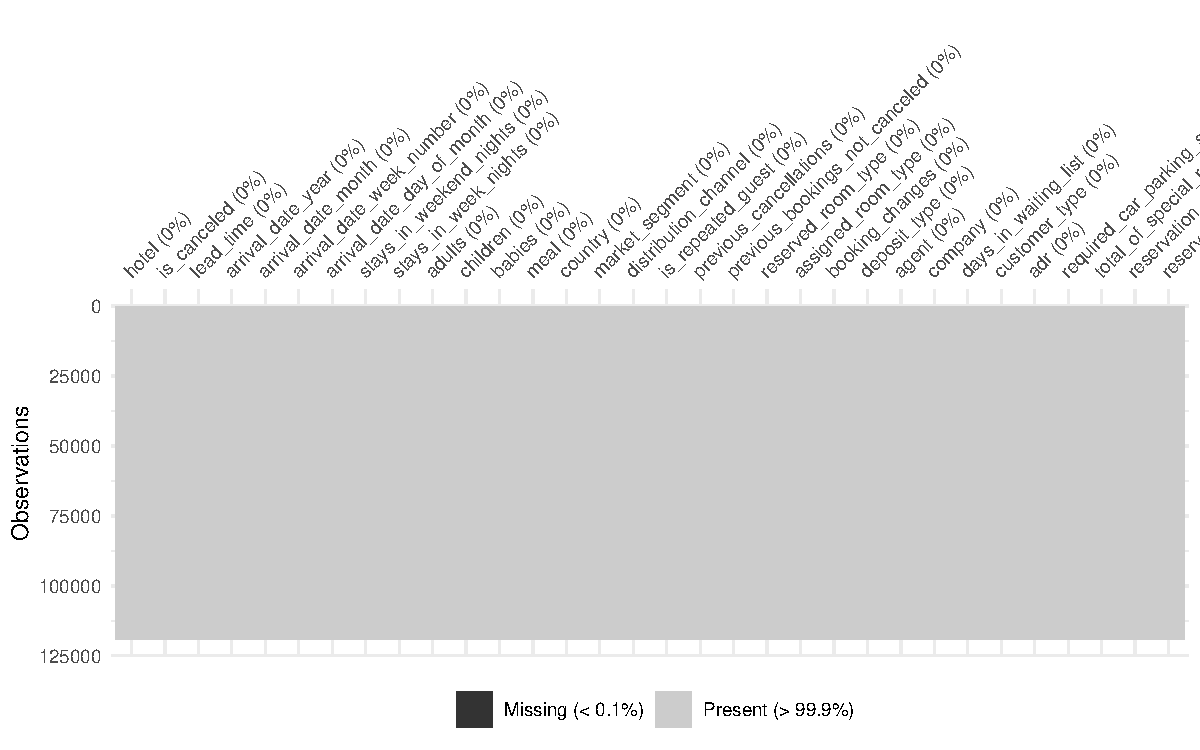
\includegraphics{tidy_files/figure-latex/check NA-1.pdf}

\begin{Shaded}
\begin{Highlighting}[]
<<<<<<< HEAD
\NormalTok{hotel <-}\StringTok{ }\KeywordTok{na.omit}\NormalTok{(hotels)}
=======
\NormalTok{hotel \textless{}{-}}\StringTok{ }\KeywordTok{na.omit}\NormalTok{(hotels)}
>>>>>>> master
\end{Highlighting}
\end{Shaded}

\begin{Shaded}
\begin{Highlighting}[]
<<<<<<< HEAD
\NormalTok{hotel <-}\StringTok{ }\NormalTok{hotel }\OperatorTok\StringTok{ }\KeywordTok{mutate}\NormalTok{(}
    \DataTypeTok{arr_date_month =} \KeywordTok{case_when}\NormalTok{(   }\CommentTok{# change Month to the numeric }
\NormalTok{    arrival_date_month}\OperatorTok{==}\StringTok{"January"} \OperatorTok{~}\StringTok{ }\DecValTok{01}\NormalTok{,}
\NormalTok{    arrival_date_month}\OperatorTok{==}\StringTok{"February"} \OperatorTok{~}\StringTok{ }\DecValTok{02}\NormalTok{,}
\NormalTok{    arrival_date_month}\OperatorTok{==}\StringTok{"March"} \OperatorTok{~}\StringTok{ }\DecValTok{03}\NormalTok{,}
\NormalTok{    arrival_date_month}\OperatorTok{==}\StringTok{"April"} \OperatorTok{~}\StringTok{ }\DecValTok{04}\NormalTok{,}
\NormalTok{    arrival_date_month}\OperatorTok{==}\StringTok{"May"} \OperatorTok{~}\StringTok{ }\DecValTok{05}\NormalTok{,}
\NormalTok{    arrival_date_month}\OperatorTok{==}\StringTok{"June"} \OperatorTok{~}\StringTok{ }\DecValTok{06}\NormalTok{,}
\NormalTok{    arrival_date_month}\OperatorTok{==}\StringTok{"July"} \OperatorTok{~}\StringTok{ }\DecValTok{07}\NormalTok{,}
\NormalTok{    arrival_date_month}\OperatorTok{==}\StringTok{"August"} \OperatorTok{~}\StringTok{ }\DecValTok{08}\NormalTok{,}
\NormalTok{    arrival_date_month}\OperatorTok{==}\StringTok{"September"} \OperatorTok{~}\StringTok{ }\DecValTok{09}\NormalTok{,}
\NormalTok{    arrival_date_month}\OperatorTok{==}\StringTok{"October"} \OperatorTok{~}\StringTok{ }\DecValTok{10}\NormalTok{,}
\NormalTok{    arrival_date_month}\OperatorTok{==}\StringTok{"November"} \OperatorTok{~}\StringTok{ }\DecValTok{11}\NormalTok{,}
\NormalTok{    arrival_date_month}\OperatorTok{==}\StringTok{"December"} \OperatorTok{~}\StringTok{ }\DecValTok{12}\NormalTok{),}
    \DataTypeTok{country =} \KeywordTok{str_replace}\NormalTok{(country, }\DataTypeTok{pattern =} \StringTok{"cn"}\NormalTok{, }\DataTypeTok{replacement =} \StringTok{"chn"}\NormalTok{), }\CommentTok{# replace China pattern}
    \DataTypeTok{deposit =} \KeywordTok{case_when}\NormalTok{(deposit_type }\OperatorTok{==}\StringTok{ "No Deposit"}\OperatorTok{~}\DecValTok{0}\NormalTok{,            }\CommentTok{# Change deposit as binary numeric}
\NormalTok{                        deposit_type }\OperatorTok{==}\StringTok{ "Non Refund"}\OperatorTok{~}\DecValTok{1}\NormalTok{,}
\NormalTok{                         deposit_type }\OperatorTok{==}\StringTok{ "Refundable"}\OperatorTok{~}\DecValTok{2}\NormalTok{),}
   \DataTypeTok{arrival_time=}\KeywordTok{paste}\NormalTok{(arrival_date_year,}
\NormalTok{                      arrival_date_month,}
\NormalTok{                      arrival_date_day_of_month,}
                      \DataTypeTok{sep=}\StringTok{"-"}\NormalTok{))}


\NormalTok{  sec_mute <-}\StringTok{ }\NormalTok{hotel }\OperatorTok\StringTok{ }\KeywordTok{mutate}\NormalTok{(}\DataTypeTok{Country =} \KeywordTok{countrycode}\NormalTok{(}\DataTypeTok{sourcevar =}\NormalTok{ country,              }\CommentTok{# According the country code to find the country full name}
                                      \DataTypeTok{origin =} \StringTok{"iso3c"}\NormalTok{,}
                                      \DataTypeTok{destination =} \StringTok{"country.name"}\NormalTok{),}
          \DataTypeTok{reservation_status_date=}\KeywordTok{ymd}\NormalTok{(reservation_status_date),}
         \DataTypeTok{arrival_time=}\KeywordTok{ymd}\NormalTok{(arrival_time)) }
=======
\NormalTok{hotel \textless{}{-}}\StringTok{ }\NormalTok{hotel }\OperatorTok{\%\textgreater{}\%}\StringTok{ }\KeywordTok{mutate}\NormalTok{(}
    \DataTypeTok{arr\_date\_month =} \KeywordTok{case\_when}\NormalTok{(   }\CommentTok{\# change Month to the numeric }
\NormalTok{    arrival\_date\_month}\OperatorTok{==}\StringTok{"January"} \OperatorTok{\textasciitilde{}}\StringTok{ }\DecValTok{01}\NormalTok{,}
\NormalTok{    arrival\_date\_month}\OperatorTok{==}\StringTok{"February"} \OperatorTok{\textasciitilde{}}\StringTok{ }\DecValTok{02}\NormalTok{,}
\NormalTok{    arrival\_date\_month}\OperatorTok{==}\StringTok{"March"} \OperatorTok{\textasciitilde{}}\StringTok{ }\DecValTok{03}\NormalTok{,}
\NormalTok{    arrival\_date\_month}\OperatorTok{==}\StringTok{"April"} \OperatorTok{\textasciitilde{}}\StringTok{ }\DecValTok{04}\NormalTok{,}
\NormalTok{    arrival\_date\_month}\OperatorTok{==}\StringTok{"May"} \OperatorTok{\textasciitilde{}}\StringTok{ }\DecValTok{05}\NormalTok{,}
\NormalTok{    arrival\_date\_month}\OperatorTok{==}\StringTok{"June"} \OperatorTok{\textasciitilde{}}\StringTok{ }\DecValTok{06}\NormalTok{,}
\NormalTok{    arrival\_date\_month}\OperatorTok{==}\StringTok{"July"} \OperatorTok{\textasciitilde{}}\StringTok{ }\DecValTok{07}\NormalTok{,}
\NormalTok{    arrival\_date\_month}\OperatorTok{==}\StringTok{"August"} \OperatorTok{\textasciitilde{}}\StringTok{ }\DecValTok{08}\NormalTok{,}
\NormalTok{    arrival\_date\_month}\OperatorTok{==}\StringTok{"September"} \OperatorTok{\textasciitilde{}}\StringTok{ }\DecValTok{09}\NormalTok{,}
\NormalTok{    arrival\_date\_month}\OperatorTok{==}\StringTok{"October"} \OperatorTok{\textasciitilde{}}\StringTok{ }\DecValTok{10}\NormalTok{,}
\NormalTok{    arrival\_date\_month}\OperatorTok{==}\StringTok{"November"} \OperatorTok{\textasciitilde{}}\StringTok{ }\DecValTok{11}\NormalTok{,}
\NormalTok{    arrival\_date\_month}\OperatorTok{==}\StringTok{"December"} \OperatorTok{\textasciitilde{}}\StringTok{ }\DecValTok{12}\NormalTok{),}
    \DataTypeTok{country =} \KeywordTok{str\_replace}\NormalTok{(country, }\DataTypeTok{pattern =} \StringTok{"cn"}\NormalTok{, }\DataTypeTok{replacement =} \StringTok{"chn"}\NormalTok{), }\CommentTok{\# replace China pattern}
    \DataTypeTok{deposit =} \KeywordTok{case\_when}\NormalTok{(deposit\_type }\OperatorTok{==}\StringTok{ "No Deposit"}\OperatorTok{\textasciitilde{}}\DecValTok{0}\NormalTok{,            }\CommentTok{\# Change deposit as binary numeric}
\NormalTok{                        deposit\_type }\OperatorTok{==}\StringTok{ "Non Refund"}\OperatorTok{\textasciitilde{}}\DecValTok{1}\NormalTok{,}
\NormalTok{                         deposit\_type }\OperatorTok{==}\StringTok{ "Refundable"}\OperatorTok{\textasciitilde{}}\DecValTok{2}\NormalTok{),}
   \DataTypeTok{arrival\_time=}\KeywordTok{paste}\NormalTok{(arrival\_date\_year,}
\NormalTok{                      arrival\_date\_month,}
\NormalTok{                      arrival\_date\_day\_of\_month,}
                      \DataTypeTok{sep=}\StringTok{"{-}"}\NormalTok{))}
\NormalTok{  sec\_mute \textless{}{-}}\StringTok{ }\NormalTok{hotel }\OperatorTok{\%\textgreater{}\%}\StringTok{ }\KeywordTok{mutate}\NormalTok{(}\DataTypeTok{Country =} \KeywordTok{countrycode}\NormalTok{(}\DataTypeTok{sourcevar =}\NormalTok{ country,              }\CommentTok{\# According the country code to find the country full name}
                                      \DataTypeTok{origin =} \StringTok{"iso3c"}\NormalTok{,}
                                      \DataTypeTok{destination =} \StringTok{"country.name"}\NormalTok{),}
          \DataTypeTok{reservation\_status\_date=}\KeywordTok{ymd}\NormalTok{(reservation\_status\_date),}
         \DataTypeTok{arrival\_time=}\KeywordTok{ymd}\NormalTok{(arrival\_time)) }
>>>>>>> master
\end{Highlighting}
\end{Shaded}

\begin{Shaded}
\begin{Highlighting}[]
<<<<<<< HEAD
\NormalTok{Miss <-}\StringTok{ }\KeywordTok{sapply}\NormalTok{(hotels, }\ControlFlowTok{function}\NormalTok{(x) }\KeywordTok{sum}\NormalTok{(}\KeywordTok{is.na}\NormalTok{(x))) }\CommentTok{# Check mssing value }
=======
\NormalTok{Miss \textless{}{-}}\StringTok{ }\KeywordTok{sapply}\NormalTok{(hotels, }\ControlFlowTok{function}\NormalTok{(x) }\KeywordTok{sum}\NormalTok{(}\KeywordTok{is.na}\NormalTok{(x))) }\CommentTok{\# Check mssing value }
>>>>>>> master
\NormalTok{Miss}
\end{Highlighting}
\end{Shaded}

\begin{verbatim}
##                          hotel                    is_canceled 
##                              0                              0 
##                      lead_time              arrival_date_year 
##                              0                              0 
##             arrival_date_month       arrival_date_week_number 
##                              0                              0 
##      arrival_date_day_of_month        stays_in_weekend_nights 
##                              0                              0 
##           stays_in_week_nights                         adults 
##                              0                              0 
##                       children                         babies 
##                              4                              0 
##                           meal                        country 
##                              0                              0 
##                 market_segment           distribution_channel 
##                              0                              0 
##              is_repeated_guest         previous_cancellations 
##                              0                              0 
## previous_bookings_not_canceled             reserved_room_type 
##                              0                              0 
##             assigned_room_type                booking_changes 
##                              0                              0 
##                   deposit_type                          agent 
##                              0                              0 
##                        company           days_in_waiting_list 
##                              0                              0 
##                  customer_type                            adr 
##                              0                              0 
##    required_car_parking_spaces      total_of_special_requests 
##                              0                              0 
##             reservation_status        reservation_status_date 
##                              0                              0
\end{verbatim}

\begin{Shaded}
\begin{Highlighting}[]
<<<<<<< HEAD
\NormalTok{vis_final <-}\StringTok{ }\KeywordTok{vis_miss}\NormalTok{(sec_mute, }\DataTypeTok{warn_large_data =}\OtherTok{FALSE}\NormalTok{)}
\NormalTok{vis_final}
\end{Highlighting}
\end{Shaded}

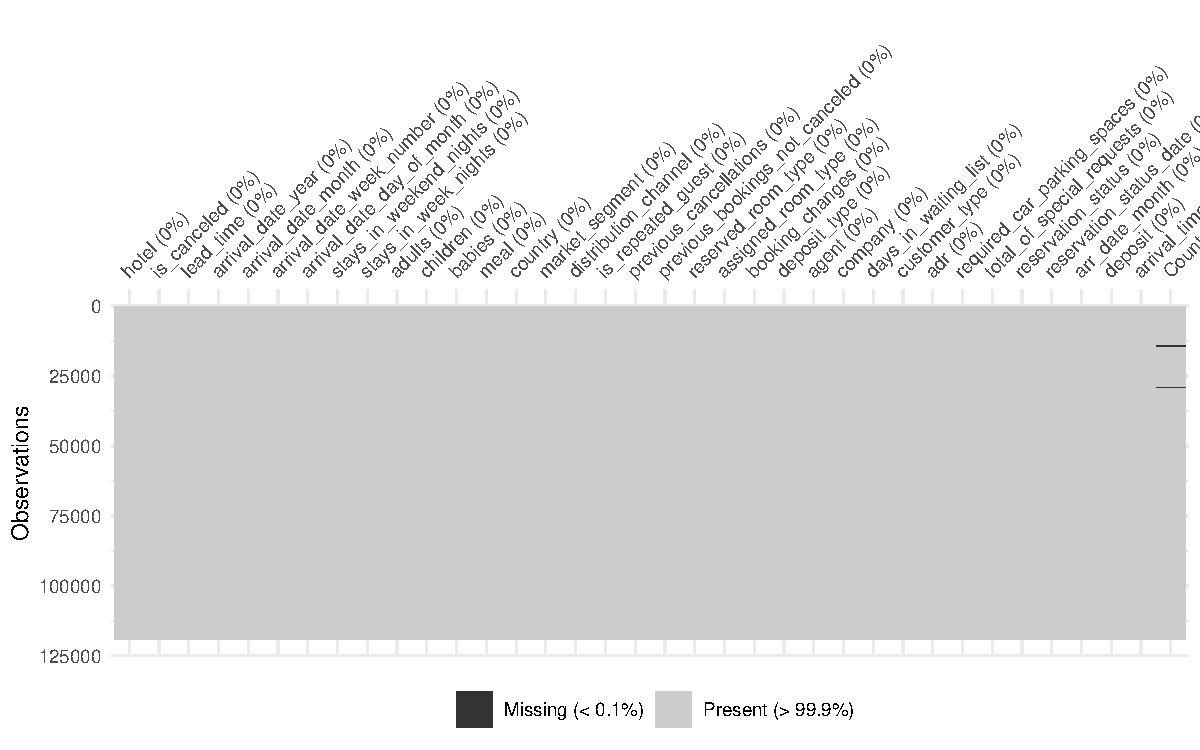
\includegraphics{tidy_files/figure-latex/secfinal-1.pdf}

\begin{Shaded}
\begin{Highlighting}[]
\NormalTok{sec_mute <-}\StringTok{ }\NormalTok{sec_mute  }\OperatorTok\StringTok{ }\NormalTok{dplyr}\OperatorTok{::}\KeywordTok{select}\NormalTok{(}\OperatorTok{-}\NormalTok{market_segment,}
                               \OperatorTok{-}\NormalTok{distribution_channel,}
                               \OperatorTok{-}\NormalTok{deposit_type,}
                               \OperatorTok{-}\NormalTok{agent,}
                               \OperatorTok{-}\NormalTok{company) }
\end{Highlighting}
\end{Shaded}

\begin{Shaded}
\begin{Highlighting}[]
\NormalTok{final <-}\StringTok{ }\KeywordTok{na.omit}\NormalTok{(sec_mute)  }\CommentTok{# Delete the missing country observations}
\end{Highlighting}
\end{Shaded}

\begin{Shaded}
\begin{Highlighting}[]
\NormalTok{bookings_table <-}\StringTok{ }\NormalTok{final }\OperatorTok
\StringTok{  }\KeywordTok{filter}\NormalTok{(}\OperatorTok{!}\NormalTok{country }\OperatorTok{==}\StringTok{ "NULL"}\NormalTok{) }\OperatorTok\StringTok{      }\CommentTok{# In some observations we don't know the country}
\StringTok{  }\KeywordTok{count}\NormalTok{(country, hotel, is_canceled)}


\CommentTok{# Let's derive some stats:}
\CommentTok{# 1. Top-10 countries with most bookings}

\NormalTok{bookings_by_countries <-}\StringTok{ }\NormalTok{bookings_table }\OperatorTok
\StringTok{  }\KeywordTok{group_by}\NormalTok{(country) }\OperatorTok
\StringTok{  }\KeywordTok{summarise}\NormalTok{(}\DataTypeTok{total_bookings =} \KeywordTok{sum}\NormalTok{(n, }\DataTypeTok{na.rm =} \OtherTok{TRUE}\NormalTok{)) }\OperatorTok
\StringTok{  }\KeywordTok{mutate}\NormalTok{(}\DataTypeTok{booking_prop =}\NormalTok{ total_bookings}\OperatorTok{/}\KeywordTok{sum}\NormalTok{(total_bookings, }\DataTypeTok{na.rm =} \OtherTok{TRUE}\NormalTok{) }\OperatorTok{*}\StringTok{ }\DecValTok{100}\NormalTok{) }\OperatorTok
\StringTok{  }\KeywordTok{arrange}\NormalTok{(}\KeywordTok{desc}\NormalTok{(total_bookings))}
\end{Highlighting}
\end{Shaded}

\begin{verbatim}
## `summarise()` ungrouping output (override with `.groups` argument)
\end{verbatim}

\begin{Shaded}
\begin{Highlighting}[]
\CommentTok{## I show this in the first figure no need to add it again}

\CommentTok{#As we expected Portugal is first the rest countreis are all in Europe except of Brazil}

\CommentTok{#Now let's calculate the proportion of this bookings in the total}




\CommentTok{# The percent in the total bookings is more interesting}

\CommentTok{# As wee see out of all bookings 40% of those come from within Portugal}

\CommentTok{# 2.  Top-10 countries with most bookings by hotel type}

\CommentTok{# Now lets see if the above proportions will be simillar among hotel types}
\CommentTok{## at the moment we don't look at the is_cancelled variable}

\NormalTok{hotel_book_prop <-}\StringTok{ }\NormalTok{bookings_table }\OperatorTok
\StringTok{  }\KeywordTok{group_by}\NormalTok{(country, hotel) }\OperatorTok
\StringTok{  }\KeywordTok{summarise}\NormalTok{(}\DataTypeTok{hotel_bookings =}  \KeywordTok{sum}\NormalTok{(n, }\DataTypeTok{na.rm =} \OtherTok{TRUE}\NormalTok{)) }\OperatorTok
\CommentTok{# we have total bookings bookings by country and now we calc. the proportion}
\StringTok{  }\KeywordTok{group_by}\NormalTok{(hotel) }\OperatorTok
\StringTok{  }\KeywordTok{mutate}\NormalTok{(}\DataTypeTok{hotel_booking_prop =}\NormalTok{ hotel_bookings}\OperatorTok{/}\KeywordTok{sum}\NormalTok{(hotel_bookings, }\DataTypeTok{na.rm =} \OtherTok{TRUE}\NormalTok{)) }\OperatorTok
\StringTok{  }\KeywordTok{arrange}\NormalTok{(hotel, }\KeywordTok{desc}\NormalTok{(hotel_booking_prop))}
\end{Highlighting}
\end{Shaded}

\begin{verbatim}
## `summarise()` regrouping output by 'country' (override with `.groups` argument)
\end{verbatim}

\begin{Shaded}
\begin{Highlighting}[]
\CommentTok{# Now that we have the table let's compare the proportions of the first 10 countries for}
\CommentTok{#each hotel type}

\NormalTok{resort_prop <-}\StringTok{ }\NormalTok{hotel_book_prop }\OperatorTok
\StringTok{  }\KeywordTok{filter}\NormalTok{(hotel }\OperatorTok{==}\StringTok{ "Resort Hotel"}\NormalTok{) }\OperatorTok
\StringTok{  }\KeywordTok{head}\NormalTok{(}\DecValTok{10}\NormalTok{)}


\NormalTok{city_prop <-}\StringTok{ }\NormalTok{hotel_book_prop }\OperatorTok
\StringTok{  }\KeywordTok{filter}\NormalTok{(hotel }\OperatorTok{==}\StringTok{ "City Hotel"}\NormalTok{) }\OperatorTok
\StringTok{  }\KeywordTok{head}\NormalTok{(}\DecValTok{10}\NormalTok{)}

\CommentTok{# The majority of the countries are the same}

\NormalTok{common_countries <-}\StringTok{   }\NormalTok{resort_prop }\OperatorTok
\StringTok{    }\KeywordTok{filter}\NormalTok{(country }\OperatorTok\StringTok{  }\NormalTok{city_prop}\OperatorTok{$}\NormalTok{country) }\OperatorTok
\StringTok{    }\KeywordTok{pull}\NormalTok{(country)}

\NormalTok{diff_countries <-}\StringTok{   }\NormalTok{resort_prop }\OperatorTok
\StringTok{  }\KeywordTok{filter}\NormalTok{(}\OperatorTok{!}\NormalTok{country }\OperatorTok\StringTok{  }\NormalTok{city_prop}\OperatorTok{$}\NormalTok{country) }\OperatorTok
\StringTok{  }\KeywordTok{pull}\NormalTok{(country)}

\NormalTok{sample_countries <-}\StringTok{ }\KeywordTok{c}\NormalTok{(common_countries, diff_countries)}



\CommentTok{# IRL is more interested in the resort hotel}

\CommentTok{# Proportion of visits in the Resort Hotel}

\NormalTok{city <-}\StringTok{ }\KeywordTok{readPNG}\NormalTok{(}\StringTok{"images/city-hotel.png"}\NormalTok{)}
\NormalTok{resort <-}\StringTok{ }\KeywordTok{readPNG}\NormalTok{(}\StringTok{"images/resort-hotel.png"}\NormalTok{)}
\end{Highlighting}
\end{Shaded}

\begin{Shaded}
\begin{Highlighting}[]
\NormalTok{book_day <-}\StringTok{ }\NormalTok{final }\OperatorTok
\StringTok{  }\KeywordTok{filter}\NormalTok{(arrival_date_year }\OperatorTok{==}\StringTok{ }\DecValTok{2017}\NormalTok{) }\OperatorTok
\StringTok{  }\KeywordTok{filter}\NormalTok{(children }\OperatorTok{==}\StringTok{ }\DecValTok{0} \OperatorTok{&}\StringTok{ }\NormalTok{babies }\OperatorTok{==}\StringTok{ }\DecValTok{0}\NormalTok{) }\OperatorTok
\StringTok{  }\KeywordTok{filter}\NormalTok{(stays_in_week_nights }\OperatorTok{==}\StringTok{ }\DecValTok{5}\NormalTok{) }\OperatorTok
\StringTok{  }\NormalTok{dplyr}\OperatorTok{::}\KeywordTok{select}\NormalTok{(reservation_status_date, adr) }\OperatorTok
\StringTok{  }\KeywordTok{arrange}\NormalTok{((adr)) }\OperatorTok
\StringTok{  }\KeywordTok{filter}\NormalTok{(adr }\OperatorTok{!=}\StringTok{ }\DecValTok{0}\NormalTok{) }\OperatorTok
\StringTok{  }\KeywordTok{head}\NormalTok{(}\DecValTok{10}\NormalTok{) }\OperatorTok
\StringTok{  }\KeywordTok{as_tibble}\NormalTok{() }\OperatorTok
\StringTok{  }\KeywordTok{mutate}\NormalTok{(}\DataTypeTok{day =} \KeywordTok{as.Date}\NormalTok{(reservation_status_date) }\OperatorTok{-}\StringTok{ }\KeywordTok{as.Date}\NormalTok{(}\KeywordTok{as.character}\NormalTok{(}\StringTok{"2017-01-01"}\NormalTok{), }\DataTypeTok{format=}\StringTok{"%Y-%m-%d"}\NormalTok{)) }\OperatorTok
\StringTok{  }\KeywordTok{filter}\NormalTok{(day }\OperatorTok{>}\StringTok{ }\DecValTok{0}\NormalTok{)}





\NormalTok{calendar <-}\StringTok{ }\KeywordTok{calendR}\NormalTok{(}\DataTypeTok{year =} \DecValTok{2017}\NormalTok{,}
        \DataTypeTok{start =} \StringTok{"M"}\NormalTok{,}
        \DataTypeTok{special.days =}\NormalTok{ book_day}\OperatorTok{$}\NormalTok{day,}
        \DataTypeTok{special.col =} \StringTok{"green"}\NormalTok{,            }\CommentTok{# Color of the specified days}
        \DataTypeTok{low.col =} \StringTok{"white"}\NormalTok{,}
        \DataTypeTok{weeknames.size =} \DecValTok{3}\NormalTok{,}
        \DataTypeTok{day.size =} \DecValTok{2}\NormalTok{,}
        \DataTypeTok{orientation =}\StringTok{"p"}\NormalTok{,}
        \DataTypeTok{title =} \StringTok{""}\NormalTok{,}
        \DataTypeTok{subtitle =} \StringTok{""}\NormalTok{) }\OperatorTok{+}
\StringTok{  }\NormalTok{tvthemes}\OperatorTok{::}\KeywordTok{theme_avatar}\NormalTok{() }\OperatorTok{+}
\StringTok{  }\KeywordTok{theme}\NormalTok{(}
    \DataTypeTok{legend.position =} \StringTok{"none"}
\NormalTok{  ) }\OperatorTok{+}
\StringTok{  }\KeywordTok{labs}\NormalTok{(}
    \DataTypeTok{title =} \StringTok{"Cheapest Day to book"}
\NormalTok{  )}
\end{Highlighting}
\end{Shaded}

\begin{Shaded}
\begin{Highlighting}[]
\NormalTok{visitors <-}\StringTok{ }\NormalTok{final }\OperatorTok
\StringTok{  }\KeywordTok{mutate}\NormalTok{(}\DataTypeTok{Date =}\NormalTok{ lubridate}\OperatorTok{::}\KeywordTok{as_date}\NormalTok{(}
    \KeywordTok{str_c}\NormalTok{(arrival_date_year,}
\NormalTok{          arrival_date_month,}
\NormalTok{          arrival_date_day_of_month,}
          \DataTypeTok{sep =} \StringTok{"/"}\NormalTok{))) }\OperatorTok
\StringTok{  }\KeywordTok{count}\NormalTok{(hotel, arrival_date_year, Date) }\OperatorTok
\StringTok{  }\KeywordTok{mutate}\NormalTok{(}\DataTypeTok{above_average =} \KeywordTok{case_when}\NormalTok{(}
\NormalTok{    n }\OperatorTok{>}\StringTok{ }\KeywordTok{mean}\NormalTok{(n) }\OperatorTok{~}\StringTok{ }\DecValTok{1}\NormalTok{,}
\NormalTok{    n }\OperatorTok{<=}\StringTok{ }\KeywordTok{mean}\NormalTok{(n) }\OperatorTok{~}\StringTok{ }\DecValTok{0}
\NormalTok{  ))}
\end{Highlighting}
\end{Shaded}

\begin{Shaded}
\begin{Highlighting}[]
\NormalTok{to_map <-}\StringTok{ }\NormalTok{final }\OperatorTok
\StringTok{    }\KeywordTok{mutate}\NormalTok{(}\DataTypeTok{Country =} \KeywordTok{as.factor}\NormalTok{(Country)) }\OperatorTok
\StringTok{    }\KeywordTok{count}\NormalTok{(Country, is_canceled) }\OperatorTok
\StringTok{    }\KeywordTok{group_by}\NormalTok{(Country) }\OperatorTok
\StringTok{    }\KeywordTok{mutate}\NormalTok{(}\DataTypeTok{total_bookings =} \KeywordTok{sum}\NormalTok{(n),}
           \DataTypeTok{perc_cancel =} \KeywordTok{case_when}\NormalTok{(}
\NormalTok{             is_canceled }\OperatorTok{==}\StringTok{ }\DecValTok{1} \OperatorTok{~}\StringTok{ }\NormalTok{n}\OperatorTok{/}\NormalTok{total_bookings}
\NormalTok{           ),}
           \DataTypeTok{perc_arrived =} \KeywordTok{case_when}\NormalTok{(}
\NormalTok{             is_canceled }\OperatorTok{==}\StringTok{ }\DecValTok{0} \OperatorTok{~}\StringTok{ }\NormalTok{n}\OperatorTok{/}\NormalTok{total_bookings}
\NormalTok{           )}
\NormalTok{    ) }\OperatorTok
\StringTok{    }\NormalTok{dplyr}\OperatorTok{::}\KeywordTok{select}\NormalTok{(Country, total_bookings, }\KeywordTok{contains}\NormalTok{(}\StringTok{"perc"}\NormalTok{)) }\OperatorTok
\StringTok{    }\KeywordTok{pivot_longer}\NormalTok{(}
      \DataTypeTok{cols =} \KeywordTok{contains}\NormalTok{(}\StringTok{"perc"}\NormalTok{),}
      \DataTypeTok{names_to =} \StringTok{"outcome"}\NormalTok{,}
      \DataTypeTok{values_to =} \StringTok{"percentage"}
\NormalTok{    ) }\OperatorTok
\StringTok{    }\KeywordTok{na.omit}\NormalTok{() }\OperatorTok
\StringTok{    }\KeywordTok{ungroup}\NormalTok{() }\OperatorTok
\StringTok{    }\KeywordTok{filter}\NormalTok{(outcome }\OperatorTok{==}\StringTok{ "perc_cancel"}\NormalTok{)}
  
  
  
  
  
  
\NormalTok{  mapCountry<-}\StringTok{ }\NormalTok{maps}\OperatorTok{::}\KeywordTok{map}\NormalTok{(}\StringTok{"world"}\NormalTok{, }\DataTypeTok{fill =} \OtherTok{TRUE}\NormalTok{, }\DataTypeTok{plot =} \OtherTok{FALSE}\NormalTok{)}
  
  
  \KeywordTok{match}\NormalTok{(mapCountry}\OperatorTok{$}\NormalTok{names, final}\OperatorTok{$}\NormalTok{Country)}
\end{Highlighting}
\end{Shaded}

\begin{verbatim}
##    [1]  90654     NA   2215     NA  91324    647     NA     NA     NA   7097
##   [11]     NA     NA     NA     NA   5003     NA     NA     NA     NA     54
##   [21]     NA  18097     NA     NA     NA     NA     NA     NA     NA     NA
##   [31]     NA     NA     NA     NA     NA     NA     NA     NA     NA     NA
##   [41]     NA     NA     NA     NA     NA     NA     NA     NA     NA     NA
##   [51]     NA     NA     NA     NA     NA     NA     NA     NA     NA     NA
##   [61]     NA     NA     NA     NA     NA     NA     NA     NA     NA     NA
##   [71]     NA     NA     NA     NA     NA     NA     NA     NA     NA     NA
##   [81]     NA     NA     NA     NA     NA     NA     NA     NA     NA     NA
##   [91]     NA     NA     NA     NA     NA     NA     NA     NA     NA     NA
##  [101]     NA     NA     NA     NA     NA     NA     NA     NA     NA     NA
##  [111]     NA     NA     NA     NA     NA     NA     NA     NA     NA     NA
##  [121]  98040     NA     NA     NA     NA     NA     NA     NA     NA     NA
##  [131]     NA     NA     NA     NA     NA     NA     NA     NA     NA     NA
##  [141]     NA     NA     NA     NA     NA     NA     NA     NA     NA     NA
##  [151]     NA     NA     NA     NA     NA     NA     NA     NA     NA     NA
##  [161]     NA     NA     NA     NA     NA     NA     NA     NA     NA     NA
##  [171]     NA     NA     NA     NA     NA     NA    256     NA     NA     NA
##  [181]   2026     NA     NA  13389     NA  23396     93  53379  81654     NA
##  [191]     NA     NA     NA     NA     NA  48383  21248  13631     NA     NA
##  [201]     NA     NA     NA     NA     NA     NA     NA     NA     NA     NA
##  [211]     NA     NA     NA     NA     NA   2044     NA     NA     NA     NA
##  [221]  86929     NA     NA     NA     NA     NA     NA     NA     NA     NA
##  [231]     NA     NA     NA     NA     NA     NA     NA    309  90281     NA
##  [241]     NA     NA    492   8189     NA     NA     NA     NA     NA     NA
##  [251]     NA     NA     NA     NA     NA     NA     NA     NA     NA     NA
##  [261]     NA     NA     NA     NA     NA     NA     NA     NA     NA     NA
##  [271]     NA     NA     NA     NA     NA     NA     NA     NA     NA     NA
##  [281]     NA     NA     NA     NA     NA     NA     NA     NA     NA     NA
##  [291]     NA     NA     NA     NA     NA     NA     NA     NA     NA     NA
##  [301]     NA     NA     NA     NA     NA     NA     NA     NA     NA     NA
##  [311]     NA     NA     NA     NA     NA     NA     NA     NA     NA     NA
##  [321]     NA     NA     NA     NA     NA     NA     NA     NA     NA     NA
##  [331]     NA     NA     NA     NA     NA     NA     NA     NA     NA     NA
##  [341]     NA     NA     NA     NA     NA     NA     NA     NA     NA     NA
##  [351]     NA     NA     NA     NA     NA     NA     NA     NA     NA     NA
##  [361]     NA     NA     NA     NA     NA     NA     NA     NA     NA     NA
##  [371]     NA     NA     NA     NA     NA     NA     NA     NA     NA     NA
##  [381]     NA     NA     NA     NA     NA    110     NA     NA     NA     NA
##  [391]     NA     NA     NA     NA     NA     NA     NA     NA     NA     NA
##  [401]     NA     NA     NA     NA     NA     NA     NA     NA     NA     NA
##  [411]     NA     NA     NA     NA     NA     NA   1811     NA     NA     NA
##  [421]     NA     NA     NA     NA     NA     NA     NA     NA     NA    949
##  [431]     NA     NA  19258     NA     NA     NA     NA   9245     NA     NA
##  [441]     NA     NA     NA     NA     NA     NA     NA     NA     NA   3593
##  [451]     NA     NA     NA     NA     NA     NA  19153     NA     NA     NA
##  [461]     NA     NA   8193     NA     NA     NA     NA     NA     78     NA
##  [471]  37384  92949     NA     NA     NA     NA     NA     NA     NA     NA
##  [481]     NA     NA     NA    226  16925   2902     NA     NA     NA     NA
##  [491]     NA     NA     NA     NA  30207  26669     NA     NA     NA     NA
##  [501]     NA     NA     NA     NA     NA     NA     NA     NA     NA     NA
##  [511]     14     NA     NA     NA    263  44965     NA     NA     NA     NA
##  [521]     NA     NA     NA    337     NA     NA     NA     NA     NA     NA
##  [531]     NA     NA     NA     NA     NA     NA     NA     NA     NA     NA
##  [541]     NA     NA     NA     NA     NA     NA     NA     NA     NA  69564
##  [551]     NA     NA     NA     NA     NA     NA     NA     19     NA     NA
##  [561]     NA     NA     NA     NA     NA     NA     NA     NA  56014     NA
##  [571]     NA     NA     NA     NA     NA     NA     NA     NA     NA     NA
##  [581]     NA     NA     NA     NA     NA     NA     NA     NA     NA     NA
##  [591]     NA     NA   7031   9455  58758     NA     NA     NA     NA     NA
##  [601]     NA     NA     NA  62758     NA     NA     NA     NA     NA     NA
##  [611]     NA     NA     NA     NA     NA     NA     NA     NA     NA     NA
##  [621]     NA     NA     NA     NA     NA     NA     NA     NA     NA     NA
##  [631]     NA     NA     NA     NA     NA     NA     NA     NA     NA     NA
##  [641]     NA     NA     NA     NA     NA    170     NA     NA     NA     NA
##  [651]     NA     NA     NA     NA     NA     NA     NA     NA     NA     NA
##  [661]     NA     NA     NA     NA 102571     NA  97889     NA     NA     NA
##  [671]     NA  46236     NA     NA     NA     NA     NA     NA     NA     NA
##  [681]     NA     NA     NA     NA     NA     NA   6559     NA     NA     NA
##  [691]   4097     NA     NA     NA     NA     NA     NA     NA     NA     NA
##  [701]     NA     NA     NA     NA     NA     NA     NA     NA     NA     NA
##  [711]     NA     NA     NA     NA     NA     NA     NA     NA     NA     NA
##  [721]     NA     NA     NA     NA     NA     NA     NA     NA     NA     NA
##  [731]     NA     NA     NA     NA     NA     NA     NA     NA     NA     NA
##  [741]     NA     NA     NA     NA     NA     NA     NA     NA     NA     NA
##  [751]     NA     NA     NA     NA     NA     NA     NA     NA     NA     NA
##  [761]     NA     NA     NA     NA     NA     NA     NA     NA     NA     NA
##  [771]     NA     NA     NA     NA     NA     NA     NA     NA     NA     NA
##  [781]     NA     NA     NA     NA     NA     NA     NA     NA     NA     NA
##  [791]     NA     NA     NA     NA     NA     NA     NA     NA     NA     NA
##  [801]     NA     NA     NA     NA     NA     NA     NA     NA     NA     NA
##  [811]     NA     NA     NA     NA     NA     NA     NA     NA     NA     NA
##  [821]     NA     NA     NA     NA  49452     NA     NA     NA     NA     NA
##  [831]     NA     NA     NA     NA     NA     NA     NA     NA    930     NA
##  [841]     NA     NA     NA     NA     16     NA   6912  45464  31548   2313
##  [851]     NA     NA     NA     NA     NA     NA     NA    188     NA   6122
##  [861]   7925  21996     NA     NA     NA     NA     NA     NA     NA     NA
##  [871]     NA     NA     NA     NA     NA     NA     NA     NA     NA     NA
##  [881]     NA     NA     NA     NA     NA     NA     NA     NA     NA     NA
##  [891]     NA     NA     NA     NA     NA     NA     NA     NA     NA     NA
##  [901]  11770     NA  60453     NA     NA     NA     NA     NA     NA  48192
##  [911]     NA     NA     NA     NA     NA     NA     NA     NA     NA     NA
##  [921]     NA     NA     NA     NA     NA     NA     NA     NA     NA     NA
##  [931]     NA     NA     NA     NA     NA     NA     NA     NA     NA     NA
##  [941]     NA   3472     NA     NA   9645 116191  12252     NA  83191     NA
##  [951]  62508     NA     NA  18901     NA     NA   2052    506   1672     NA
##  [961]     NA   1225  48318     NA     NA     NA  31001     NA     NA     NA
##  [971]     NA     NA     NA     NA     NA     NA     NA     NA     NA     NA
##  [981]     NA     NA     NA     NA    986     NA     NA     NA     NA     NA
##  [991]     NA  85838  29134     NA     NA     NA     NA     NA     NA     NA
## [1001]     NA     NA     NA     NA     NA     NA     NA     NA     NA     NA
## [1011]     NA     NA     NA  65909     NA     NA     NA     NA     NA     NA
## [1021]     NA    491     NA     NA     NA 108346     NA  20359     NA     NA
## [1031]     NA     NA     NA     NA     NA     NA     NA     NA     NA     NA
## [1041]  86879     NA     NA     NA     NA     NA     NA     NA     NA     NA
## [1051]   9736  50918     NA     NA     NA     NA     NA     NA     NA     NA
## [1061]    202     NA     NA     NA     NA     NA     NA     NA     NA     NA
## [1071]     NA     NA     NA     NA     NA     NA     NA     NA     NA     NA
## [1081]     NA     NA     NA     NA     NA     47     NA     NA     NA     NA
## [1091]     NA     NA     NA     NA     NA     NA     NA  33888     NA     NA
## [1101]     NA     NA     NA     NA     NA     NA     NA     NA     NA     NA
## [1111]     NA     NA     NA     52     NA     NA  11923     NA     NA     NA
## [1121]     NA  78561     NA  26926     NA     NA     NA     NA     NA     NA
## [1131]     NA     NA     NA     NA     NA     NA     NA     NA     NA     NA
## [1141]     NA     NA     NA     NA     NA     NA     NA     NA     NA     NA
## [1151]     NA     NA     NA     NA     NA     NA     NA     NA     NA     NA
## [1161]     NA     NA     NA     NA     NA     NA     NA     NA     NA     NA
## [1171]     NA     NA     NA     NA     NA     NA     NA     NA     NA     NA
## [1181]     NA     NA     NA     NA     NA     NA     NA     NA     NA     NA
## [1191]     NA     NA     NA     NA     NA     NA     NA     NA     NA     NA
## [1201]     67     NA     NA   1696     NA     NA     NA     NA     NA     NA
## [1211]     NA     NA     NA     NA      1  90066     NA     NA     NA     NA
## [1221]     NA     NA     NA     NA     NA     NA     NA     NA     NA     NA
## [1231]     NA     NA     NA     NA     NA     NA     NA     NA     NA  25756
## [1241]     39     NA     NA     NA     NA     NA     NA     NA     NA     NA
## [1251]     NA     NA     NA     NA     NA     NA     NA     NA     NA     NA
## [1261]     NA     NA     NA     NA     NA     NA     NA     NA     NA     NA
## [1271]     NA     NA     NA     NA     NA     NA     NA     NA     NA     NA
## [1281]     NA     NA     NA     NA     NA     NA     NA     NA     NA     NA
## [1291]     NA     NA     NA     NA     NA     NA     NA     NA     NA     NA
## [1301]     NA     NA     NA     NA     NA     NA     NA     NA    237     NA
## [1311]     NA     NA     NA     NA     NA     NA     NA     NA     NA     NA
## [1321]     NA     NA     NA     NA     NA     NA     NA     NA     NA     NA
## [1331]     NA     NA     NA     NA     NA     NA     NA     NA     NA  46482
## [1341]     NA     NA     NA     NA  24097 112221     NA  12602  23370     NA
## [1351]     NA     NA     NA     NA     NA     NA     NA     NA     NA     NA
## [1361]     NA     NA     NA     NA     NA     NA     NA     NA     NA     NA
## [1371]     NA     NA     NA     NA     NA 115654  91654   1520     NA     NA
## [1381]     NA     NA   1698     NA     NA  20533  11316    645     NA     NA
## [1391]     NA     NA     NA    238     NA     NA     NA  22000     NA     NA
## [1401]     NA     NA  36701     NA     NA     NA     NA     NA     NA     NA
## [1411]     NA     NA  16349     NA     NA     NA     NA     NA     NA     NA
## [1421]     NA     NA     NA     NA     NA     NA     NA     NA   5459     NA
## [1431]   2157     NA     NA  37087     NA     NA     NA  55760  21102     NA
## [1441]   1504   7683     NA     NA     NA     NA     NA     NA     NA     NA
## [1451]     NA     NA     NA     NA     NA     NA     NA     NA     NA     NA
## [1461]     NA     NA     NA     NA     NA     NA     NA     NA     NA     NA
## [1471]     NA     NA     NA     NA     NA     NA     NA     NA     NA     NA
## [1481]     NA     NA     NA     NA     NA     NA     NA     NA     NA     NA
## [1491]     NA     NA     NA     NA     NA     NA     NA     NA     NA     NA
## [1501]     NA     NA     NA     NA     NA     NA     NA     NA     NA     NA
## [1511]     NA     NA     NA     NA     NA     NA     NA     NA     NA     NA
## [1521]     NA     NA     NA     NA     NA     NA     NA     NA     NA     NA
## [1531]     NA     NA     NA     NA     NA     NA     NA     NA     NA     NA
## [1541]     NA     NA     NA     NA     NA     NA     NA     NA     NA     NA
## [1551]     NA     NA     NA     NA     NA     NA     NA     NA     NA     NA
## [1561]     NA     NA     NA     NA     NA     NA     NA     NA     NA     NA
## [1571]     NA  32370     NA     NA     NA     NA     NA     NA     NA     NA
## [1581]     NA  10725     NA     NA     NA     NA     NA     NA     NA     NA
## [1591]     NA     NA     NA     NA     NA  25067     NA     NA     NA     NA
## [1601]     NA     NA     NA     NA     NA     NA     NA     NA     NA     NA
## [1611]     NA     NA     NA     NA     NA     NA     NA     NA     NA     NA
## [1621]   2200     NA   2645   2877     NA     NA     NA
\end{verbatim}

\begin{Shaded}
\begin{Highlighting}[]
\NormalTok{  pal_fun <-}\StringTok{ }\KeywordTok{colorQuantile}\NormalTok{(}\KeywordTok{rev}\NormalTok{(}\KeywordTok{brewer.pal}\NormalTok{(}\DecValTok{3}\NormalTok{,}\StringTok{"RdYlGn"}\NormalTok{)), }\OtherTok{NULL}\NormalTok{, }\DataTypeTok{n =} \DecValTok{7}\NormalTok{,)}
  
  
\NormalTok{  color_perc <-}\StringTok{ }\NormalTok{to_map}\OperatorTok{$}\NormalTok{percentage[}\KeywordTok{match}\NormalTok{(mapCountry}\OperatorTok{$}\NormalTok{names, to_map}\OperatorTok{$}\NormalTok{Country)]}
  
  
\NormalTok{  map <-}\StringTok{ }\KeywordTok{leaflet}\NormalTok{(mapCountry) }\OperatorTok\StringTok{ }\CommentTok{# create a blank canvas}
\StringTok{    }\KeywordTok{addProviderTiles}\NormalTok{(}\StringTok{"NASAGIBS.ViirsEarthAtNight2012"}\NormalTok{) }\OperatorTok
\StringTok{    }\KeywordTok{addPolygons}\NormalTok{( }\CommentTok{# draw polygons on top of the base map (tile)}
      \DataTypeTok{stroke =} \OtherTok{FALSE}\NormalTok{,}
      \DataTypeTok{smoothFactor =} \FloatTok{0.2}\NormalTok{,}
      \DataTypeTok{fillOpacity =} \DecValTok{1}\NormalTok{,}
      \DataTypeTok{color =} \OperatorTok{~}\KeywordTok{pal_fun}\NormalTok{(color_perc) }\CommentTok{# use the rate of each state to find the correct color}
\NormalTok{    )}
\NormalTok{  map}
\end{Highlighting}
\end{Shaded}

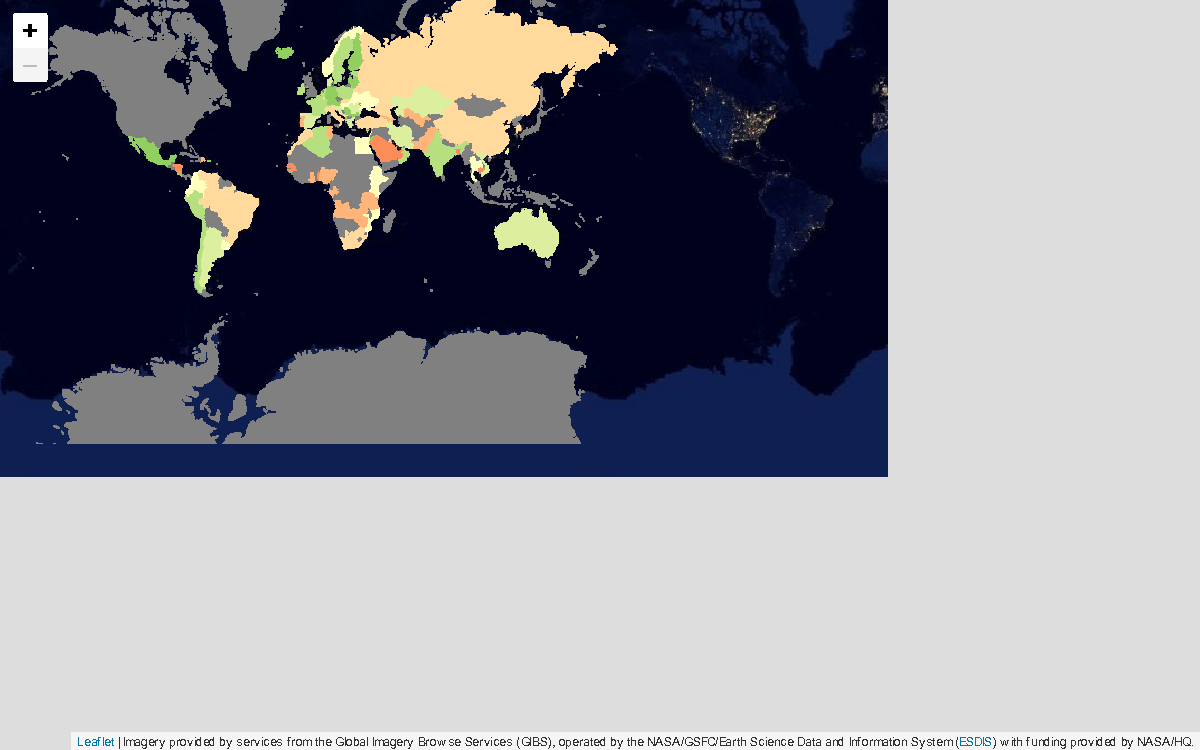
\includegraphics{tidy_files/figure-latex/unnamed-chunk-6-1.pdf}

\begin{Shaded}
\begin{Highlighting}[]
\NormalTok{pictogram <-}\StringTok{ }\NormalTok{final }\OperatorTok
\StringTok{  }\KeywordTok{count}\NormalTok{(hotel, arrival_date_month, adults, children, babies) }\OperatorTok
\StringTok{  }\KeywordTok{pivot_longer}\NormalTok{(}\DataTypeTok{cols =} \KeywordTok{c}\NormalTok{(}\StringTok{"adults"}\NormalTok{, }\StringTok{"children"}\NormalTok{, }\StringTok{"babies"}\NormalTok{),}
               \DataTypeTok{names_to =} \StringTok{"group"}\NormalTok{,}
               \DataTypeTok{values_to =} \StringTok{"number"}\NormalTok{) }\OperatorTok
\StringTok{  }\KeywordTok{group_by}\NormalTok{(hotel, arrival_date_month, group) }\OperatorTok
\StringTok{  }\KeywordTok{summarise}\NormalTok{(}\DataTypeTok{total  =} \KeywordTok{sum}\NormalTok{(number)) }\OperatorTok
\StringTok{  }\KeywordTok{filter}\NormalTok{(arrival_date_month }\OperatorTok{==}\StringTok{ "October"}\NormalTok{,}
\NormalTok{         hotel }\OperatorTok{==}\StringTok{ "Resort Hotel"}\NormalTok{) }\OperatorTok
\StringTok{  }\KeywordTok{arrange}\NormalTok{(group) }\OperatorTok
\StringTok{  }\KeywordTok{ggplot}\NormalTok{(}\KeywordTok{aes}\NormalTok{(}\DataTypeTok{label =}\NormalTok{ group, }\DataTypeTok{values =}\NormalTok{ total)) }\OperatorTok{+}
\StringTok{  }\KeywordTok{geom_pictogram}\NormalTok{(}\DataTypeTok{n_rows =} \DecValTok{10}\NormalTok{, }\KeywordTok{aes}\NormalTok{(}\DataTypeTok{colour =}\NormalTok{ group), }\DataTypeTok{flip =} \OtherTok{TRUE}\NormalTok{, }\DataTypeTok{make_proportional =} \OtherTok{TRUE}\NormalTok{) }\OperatorTok{+}
\StringTok{  }\KeywordTok{scale_color_manual}\NormalTok{(}
    \DataTypeTok{name =} \OtherTok{NULL}\NormalTok{,}
    \DataTypeTok{values =} \KeywordTok{c}\NormalTok{(}\StringTok{"#a40000"}\NormalTok{, }\StringTok{"#c68958"}\NormalTok{, }\StringTok{"#ae6056"}\NormalTok{),}
    \DataTypeTok{labels =} \KeywordTok{c}\NormalTok{(}\StringTok{"Adult"}\NormalTok{, }\StringTok{"Baby"}\NormalTok{, }\StringTok{"Child"}\NormalTok{)}
\NormalTok{  ) }\OperatorTok{+}
\StringTok{  }\KeywordTok{scale_label_pictogram}\NormalTok{(}
    \DataTypeTok{name =} \OtherTok{NULL}\NormalTok{,}
    \DataTypeTok{values =} \KeywordTok{c}\NormalTok{( }\StringTok{"female"}\NormalTok{, }\StringTok{"baby-carriage"}\NormalTok{, }\StringTok{"child"}\NormalTok{),}
    \DataTypeTok{labels =} \KeywordTok{c}\NormalTok{(}\StringTok{"Adult"}\NormalTok{, }\StringTok{"Baby"}\NormalTok{, }\StringTok{"Child"}\NormalTok{)}
\NormalTok{  ) }\OperatorTok{+}
\StringTok{  }\KeywordTok{coord_equal}\NormalTok{() }\OperatorTok{+}
\StringTok{  }\KeywordTok{theme_enhance_waffle}\NormalTok{() }\OperatorTok{+}
\StringTok{  }\KeywordTok{theme}\NormalTok{(}\DataTypeTok{legend.key.height =} \KeywordTok{unit}\NormalTok{(}\FloatTok{2.25}\NormalTok{, }\StringTok{"line"}\NormalTok{)) }\OperatorTok{+}
\StringTok{  }\KeywordTok{theme}\NormalTok{(}\DataTypeTok{legend.text =} \KeywordTok{element_text}\NormalTok{(}\DataTypeTok{size =} \DecValTok{10}\NormalTok{, }\DataTypeTok{hjust =} \DecValTok{0}\NormalTok{, }\DataTypeTok{vjust =} \FloatTok{0.75}\NormalTok{))}
\end{Highlighting}
\end{Shaded}

\begin{verbatim}
## `summarise()` regrouping output by 'hotel', 'arrival_date_month' (override with `.groups` argument)
\end{verbatim}

\begin{Shaded}
\begin{Highlighting}[]
\NormalTok{reg_data <-}\StringTok{ }\NormalTok{final }\OperatorTok
\StringTok{  }\KeywordTok{mutate}\NormalTok{(}\DataTypeTok{total_youth =}\NormalTok{ children }\OperatorTok{+}\StringTok{ }\NormalTok{babies,}
         \DataTypeTok{stay_length =}\NormalTok{ stays_in_week_nights }\OperatorTok{+}\StringTok{ }\NormalTok{stays_in_weekend_nights,}
         \DataTypeTok{family =} \KeywordTok{case_when}\NormalTok{(}
\NormalTok{           total_youth }\OperatorTok{==}\StringTok{ }\DecValTok{0} \OperatorTok{~}\StringTok{ "Without children"}\NormalTok{,}
\NormalTok{           total_youth }\OperatorTok{>}\StringTok{ }\DecValTok{0} \OperatorTok{~}\StringTok{ "With children"}\NormalTok{),}
         \DataTypeTok{visitor_type =} \KeywordTok{case_when}\NormalTok{(}
\NormalTok{           stay_length }\OperatorTok{<=}\StringTok{ }\DecValTok{2} \OperatorTok{~}\StringTok{ "max 2 days"}\NormalTok{,}
\NormalTok{           stay_length }\OperatorTok{>}\StringTok{ }\DecValTok{2} \OperatorTok{&}\StringTok{ }\NormalTok{stay_length }\OperatorTok{<=}\StringTok{ }\DecValTok{5}  \OperatorTok{~}\StringTok{ "max 5 days"}\NormalTok{,}
\NormalTok{           stay_length }\OperatorTok{>}\StringTok{ }\DecValTok{5} \OperatorTok{&}\StringTok{ }\NormalTok{stay_length }\OperatorTok{<=}\StringTok{ }\DecValTok{7}  \OperatorTok{~}\StringTok{ "max 7 days"}\NormalTok{,}
\NormalTok{           stay_length }\OperatorTok{>}\StringTok{ }\DecValTok{7} \OperatorTok{~}\StringTok{ "more than 7 days"}\NormalTok{)}
\NormalTok{  )}


\NormalTok{mod <-}\StringTok{ }\KeywordTok{glm}\NormalTok{(is_canceled }\OperatorTok{~}\StringTok{ }\NormalTok{stay_length }\OperatorTok{+}\StringTok{ }\NormalTok{total_youth, }\DataTypeTok{data =}\NormalTok{ reg_data)}


\NormalTok{mod_aug <-mod }\OperatorTok
\StringTok{  }\NormalTok{broom}\OperatorTok{::}\KeywordTok{augment}\NormalTok{(}\DataTypeTok{type.predict =} \StringTok{"response"}\NormalTok{) }\OperatorTok
\StringTok{  }\KeywordTok{mutate}\NormalTok{(}\DataTypeTok{y_hat =}\NormalTok{ .fitted)}


\NormalTok{log <-}\StringTok{ }\KeywordTok{ggplot}\NormalTok{(mod_aug, }\KeywordTok{aes}\NormalTok{(}\DataTypeTok{x =}\NormalTok{ stay_length, }\DataTypeTok{y =}\NormalTok{ y_hat)) }\OperatorTok{+}
\StringTok{  }\KeywordTok{geom_point}\NormalTok{() }\OperatorTok{+}
\StringTok{  }\KeywordTok{geom_line}\NormalTok{() }\OperatorTok{+}
\StringTok{  }\KeywordTok{scale_y_continuous}\NormalTok{(}\StringTok{"Probability of cancelling booking"}\NormalTok{, }\DataTypeTok{limits =} \KeywordTok{c}\NormalTok{(}\DecValTok{0}\NormalTok{, }\DecValTok{1}\NormalTok{))}
\end{Highlighting}
\end{Shaded}

\begin{center}\rule{0.5\linewidth}{0.5pt}\end{center}

1.What is the percentage of customer's type who book a hotel?
the transient customer is 89613, which is 74.682\%
the transient-party customer is 25120, which is 21.04\%
the contract customer is 4079,which is 3.416\%
the group customer is 577, which is 0.48\%.

\begin{Shaded}
\begin{Highlighting}[]
\NormalTok{dt1 <-final }\OperatorTok
\StringTok{  }\NormalTok{dplyr}\OperatorTok{::}\KeywordTok{select}\NormalTok{(hotel,customer_type) }\OperatorTok
\StringTok{  }\KeywordTok{count}\NormalTok{(customer_type)}

\CommentTok{# dt1 = dt1[order(dt1$n, decreasing = TRUE),]   }
\CommentTok{# myLabel = as.vector(dt1$customer_type)   }
\CommentTok{# #myLabel = paste(myLabel, "(", round(dt$n / sum(dt$n) * 100, 2), "%)", sep = "")   }

\CommentTok{# }
\CommentTok{# pp = ggplot(dt, aes(x = "", y = n, fill = customer_type)) +}
\CommentTok{#   geom_bar(stat = "identity", width = 0.5) +  }
\CommentTok{#   coord_polar(theta = "y") + }
\CommentTok{#   theme_bw() + }
\CommentTok{#   labs(x = "", y = "", title = "") + }
\CommentTok{#   theme(axis.ticks = element_blank()) + }
\CommentTok{#   #theme(legend.position = "none") + }
\CommentTok{#   theme(legend.title = element_blank(), legend.position = "left")+}
\CommentTok{#   #geom_text(aes(y = n/20 + c(0, cumsum(n)[-length(n)]), x = sum(n)/20, label = myLabel), size = 2)+}
\CommentTok{#   #geom_text(vjust=0.3,hjust=0.4)+}
\CommentTok{#   theme(axis.text.x = element_blank()) + }
\CommentTok{#   theme(panel.grid=element_blank()) +   }
\CommentTok{#   theme(panel.border=element_blank())+}
\CommentTok{#   labs(title = "the presentage of customer type")}
\CommentTok{# pp}
\CommentTok{# }
\CommentTok{#  }
\end{Highlighting}
\end{Shaded}

2.People staying in hotels tend to be one person, couples, or multiple people?
It can be seen from this figture that no matter what kind of hotel, the number of people staying in two is the most, followed by the hotel where one person stays, and the number of people staying in a family is the least.
Therefore, it is recommended that the hotel, in terms of room type arrangements, should be mainly double rooms or couple rooms. Secondly, arrange single suites. This can maximize the hotel's space utilization and maximize revenue.

\begin{Shaded}
\begin{Highlighting}[]
\NormalTok{age1<-}\StringTok{ }\NormalTok{final}\OperatorTok
\StringTok{  }\NormalTok{dplyr}\OperatorTok{::}\KeywordTok{select}\NormalTok{(hotel,adults,children,babies) }\OperatorTok
\StringTok{  }\KeywordTok{filter}\NormalTok{(hotel}\OperatorTok{==}\StringTok{"Resort Hotel"}\NormalTok{) }\OperatorTok
\StringTok{  }\KeywordTok{mutate}\NormalTok{(}\DataTypeTok{all=}\NormalTok{adults}\OperatorTok{+}\NormalTok{children}\OperatorTok{+}\NormalTok{babies)}

\NormalTok{q1<-}\KeywordTok{ggplot}\NormalTok{(age1, }\KeywordTok{aes}\NormalTok{(}\DataTypeTok{x =}\NormalTok{ all))}\OperatorTok{+}
\StringTok{  }\KeywordTok{geom_density}\NormalTok{(}\DataTypeTok{fill=}\StringTok{"green"}\NormalTok{)}\OperatorTok{+}
\StringTok{  }\KeywordTok{xlim}\NormalTok{(}\DecValTok{0}\NormalTok{,}\DecValTok{5}\NormalTok{)}\OperatorTok{+}
\StringTok{  }\KeywordTok{xlab}\NormalTok{(}\StringTok{"the number of customers in resort-hotel"}\NormalTok{) }\OperatorTok{+}
\StringTok{  }\KeywordTok{labs}\NormalTok{(}\DataTypeTok{title =} \StringTok{"the density plot in resort-hotel"}\NormalTok{)}

\NormalTok{age2<-}\StringTok{ }\NormalTok{final}\OperatorTok
\StringTok{ }\NormalTok{dplyr}\OperatorTok{::}\KeywordTok{select}\NormalTok{(hotel,adults,children,babies) }\OperatorTok
\StringTok{  }\KeywordTok{filter}\NormalTok{(hotel}\OperatorTok{==}\StringTok{"City Hotel"}\NormalTok{) }\OperatorTok
\StringTok{  }\KeywordTok{mutate}\NormalTok{(}\DataTypeTok{all=}\NormalTok{adults}\OperatorTok{+}\NormalTok{children}\OperatorTok{+}\NormalTok{babies)}

\NormalTok{q2<-}\KeywordTok{ggplot}\NormalTok{(age2, }\KeywordTok{aes}\NormalTok{(}\DataTypeTok{x =}\NormalTok{ all))}\OperatorTok{+}
\StringTok{  }\KeywordTok{geom_density}\NormalTok{(}\DataTypeTok{fill=}\StringTok{"red"}\NormalTok{)}\OperatorTok{+}
\StringTok{  }\KeywordTok{xlim}\NormalTok{(}\DecValTok{0}\NormalTok{,}\DecValTok{5}\NormalTok{)}\OperatorTok{+}
\StringTok{  }\KeywordTok{xlab}\NormalTok{(}\StringTok{"the number of customers in city-hotel"}\NormalTok{) }\OperatorTok{+}
\StringTok{  }\KeywordTok{labs}\NormalTok{(}\DataTypeTok{title =} \StringTok{"the density plot in city-hotel"}\NormalTok{)}

\KeywordTok{grid.arrange}\NormalTok{(q2, q1, }\DataTypeTok{ncol =} \DecValTok{2}\NormalTok{)}
\end{Highlighting}
\end{Shaded}

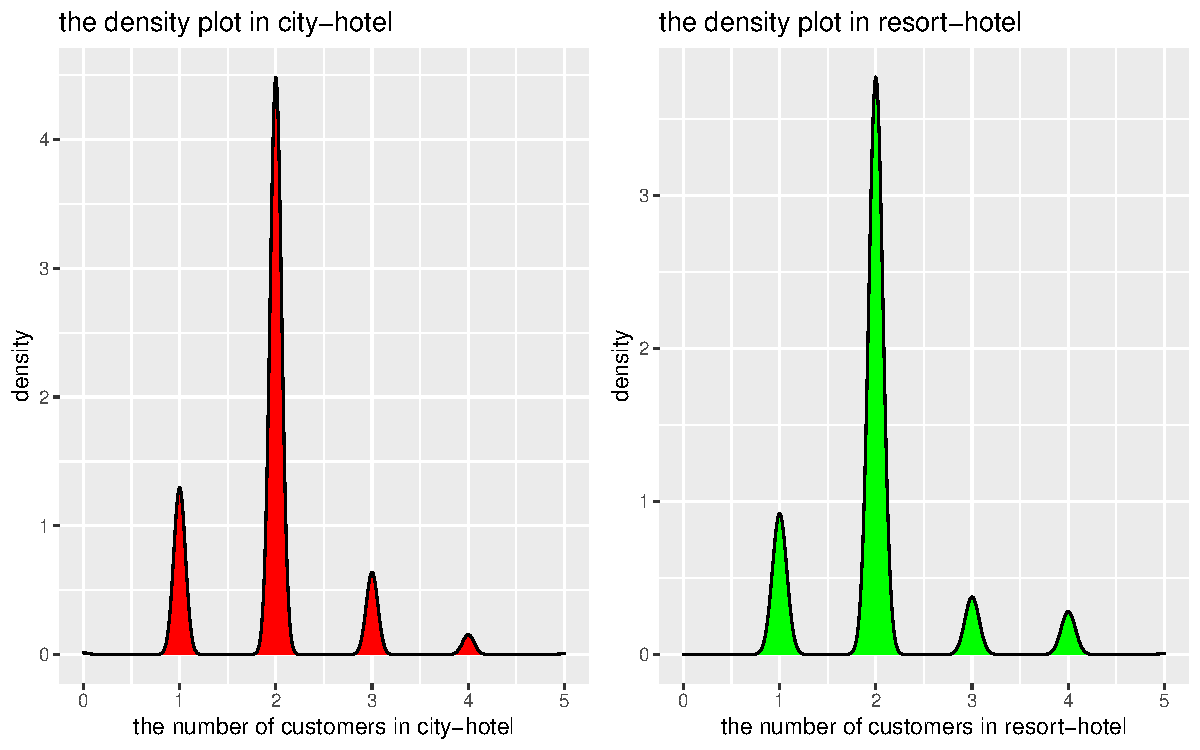
\includegraphics{tidy_files/figure-latex/the density plot by number of customers-1.pdf}

3.How long do people book hotels in advance?
The picture describes how long people tend to book a hotel in advance. The blue line is his average value (one hundred days in advance). The picture shows that hotel guests are mostly temporary hotels, while customers in city hotels Book more in advance.
Therefore, our suggestion is that for resort hotels, they should be more inclined to offline promotion, such as large physical billboards, luxurious exterior decorations, and shiny lights.
For city hotels, online advertising should be promoted, because people book more in advance, so online advertising and some coupons can attract customers more accurately.

\begin{Shaded}
\begin{Highlighting}[]
\NormalTok{ltime <-}\StringTok{ }\NormalTok{final }\OperatorTok
\StringTok{ }\NormalTok{dplyr}\OperatorTok{::}\StringTok{ }\KeywordTok{select}\NormalTok{(hotel,lead_time) }
  
\NormalTok{q3<-}\KeywordTok{ggplot}\NormalTok{(ltime, }\KeywordTok{aes}\NormalTok{(}\DataTypeTok{x =}\NormalTok{lead_time))}\OperatorTok{+}
\StringTok{  }\KeywordTok{geom_density}\NormalTok{(}\KeywordTok{aes}\NormalTok{(}\DataTypeTok{color=}\NormalTok{hotel),}\DataTypeTok{alpha=}\FloatTok{0.4}\NormalTok{)}\OperatorTok{+}
\StringTok{  }\KeywordTok{geom_vline}\NormalTok{(}\DataTypeTok{xintercept =} \KeywordTok{mean}\NormalTok{(ltime}\OperatorTok{$}\NormalTok{lead_time),}\DataTypeTok{color=}\StringTok{"blue"}\NormalTok{, }\DataTypeTok{linetype=}\StringTok{"dashed"}\NormalTok{)}\OperatorTok{+}
\StringTok{  }\KeywordTok{labs}\NormalTok{(}\DataTypeTok{title =} \StringTok{"the density of booking hotel days in advance"}\NormalTok{)}\OperatorTok{+}
\StringTok{  }\KeywordTok{xlab}\NormalTok{(}\StringTok{"the number of day booking hotel in advance"}\NormalTok{)}
\NormalTok{q3}
\end{Highlighting}
\end{Shaded}

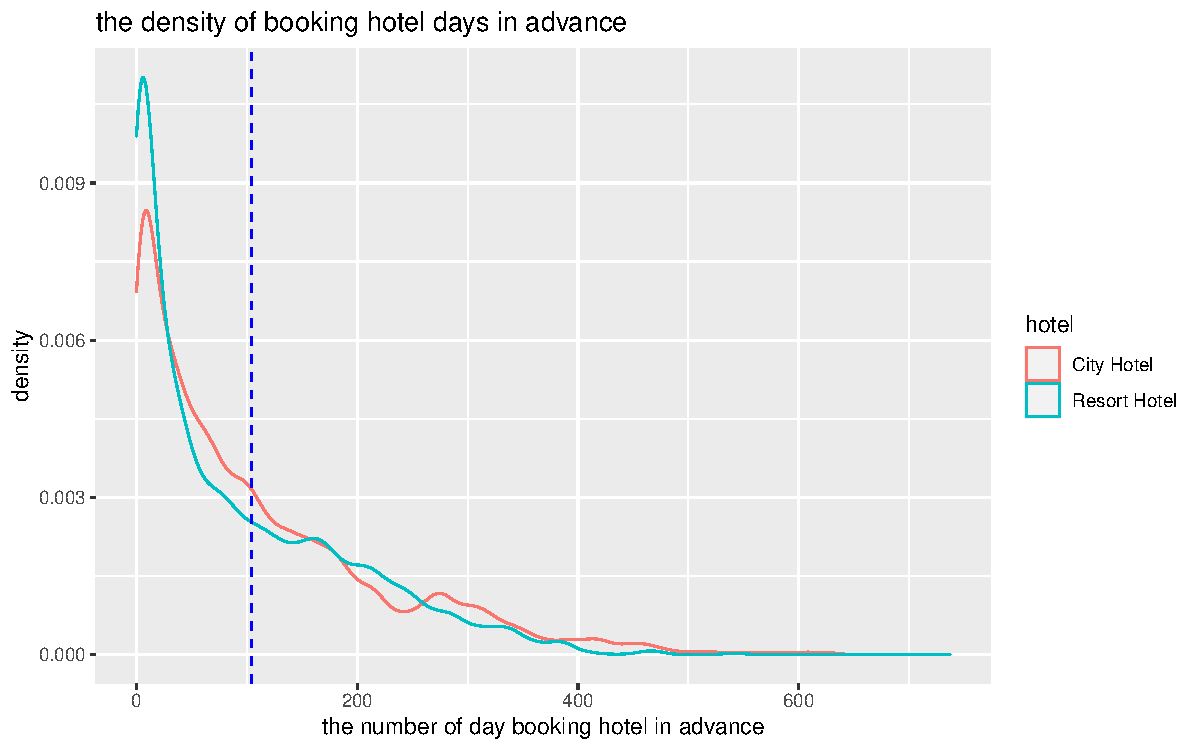
\includegraphics{tidy_files/figure-latex/leadtime-1.pdf}

This graph shows the frequency of people staying in hotels on weekends and weekdays. On weekdays, more people choose to stay for 1 to 3 nights. The average number is 2 nights. On weekends, people also choose to stay for 1 night. The number of people is more, followed by 2 nights. All in all, the proportion of customers renewing on Sunday is 2/1, while the proportion of customers renewing on weekdays is 2/5.
Therefore, we recommend that hotels do more promotional activities during workdays to increase hotel occupancy rates and renewal rates during workdays.

\begin{Shaded}
\begin{Highlighting}[]
\NormalTok{night <-}\StringTok{ }\NormalTok{final  }\OperatorTok
\StringTok{  }\NormalTok{dplyr}\OperatorTok{::}\KeywordTok{select}\NormalTok{(hotel,stays_in_week_nights) }
  
\NormalTok{n<-}\KeywordTok{ggplot}\NormalTok{(night, }\KeywordTok{aes}\NormalTok{(}\DataTypeTok{x =}\NormalTok{stays_in_week_nights))}\OperatorTok{+}
\StringTok{  }\KeywordTok{geom_density}\NormalTok{(}\KeywordTok{aes}\NormalTok{(}\DataTypeTok{color=}\NormalTok{stays_in_week_nights),}\DataTypeTok{fill=}\StringTok{"red3"}\NormalTok{,}\DataTypeTok{alpha=}\FloatTok{0.4}\NormalTok{)}\OperatorTok{+}
\StringTok{  }\KeywordTok{geom_vline}\NormalTok{(}\DataTypeTok{xintercept =} \KeywordTok{mean}\NormalTok{(night}\OperatorTok{$}\NormalTok{stays_in_week_nights),}\DataTypeTok{color=}\StringTok{"blue"}\NormalTok{, }\DataTypeTok{linetype=}\StringTok{"dashed"}\NormalTok{)}\OperatorTok{+}
\StringTok{  }\KeywordTok{xlim}\NormalTok{(}\DecValTok{0}\NormalTok{,}\DecValTok{20}\NormalTok{)}\OperatorTok{+}
\StringTok{  }\KeywordTok{labs}\NormalTok{(}\DataTypeTok{title =} \StringTok{"Number of days to stay in the hotel on weekdays"}\NormalTok{)}

\NormalTok{night1 <-}\StringTok{ }\NormalTok{final }\OperatorTok
\StringTok{  }\NormalTok{dplyr}\OperatorTok{::}\KeywordTok{select}\NormalTok{(hotel,stays_in_weekend_nights) }
  
\NormalTok{n1<-}\KeywordTok{ggplot}\NormalTok{(night1, }\KeywordTok{aes}\NormalTok{(}\DataTypeTok{x =}\NormalTok{stays_in_weekend_nights))}\OperatorTok{+}
\StringTok{  }\KeywordTok{geom_density}\NormalTok{(}\KeywordTok{aes}\NormalTok{(}\DataTypeTok{color=}\NormalTok{stays_in_weekend_nights),}\DataTypeTok{fill=}\StringTok{"green3"}\NormalTok{,}\DataTypeTok{alpha=}\FloatTok{0.4}\NormalTok{)}\OperatorTok{+}
\StringTok{  }\KeywordTok{geom_vline}\NormalTok{(}\DataTypeTok{xintercept =} \KeywordTok{mean}\NormalTok{(night1}\OperatorTok{$}\NormalTok{stays_in_weekend_nights),}\DataTypeTok{color=}\StringTok{"blue"}\NormalTok{, }\DataTypeTok{linetype=}\StringTok{"dashed"}\NormalTok{)}\OperatorTok{+}
\StringTok{  }\KeywordTok{xlim}\NormalTok{(}\DecValTok{0}\NormalTok{,}\DecValTok{10}\NormalTok{)}\OperatorTok{+}
\StringTok{  }\KeywordTok{labs}\NormalTok{(}\DataTypeTok{title =} \StringTok{"Number of days to stay in the hotel on weekdays"}\NormalTok{)}

\KeywordTok{grid.arrange}\NormalTok{(n, n1, }\DataTypeTok{ncol =} \DecValTok{1}\NormalTok{)}
\end{Highlighting}
\end{Shaded}

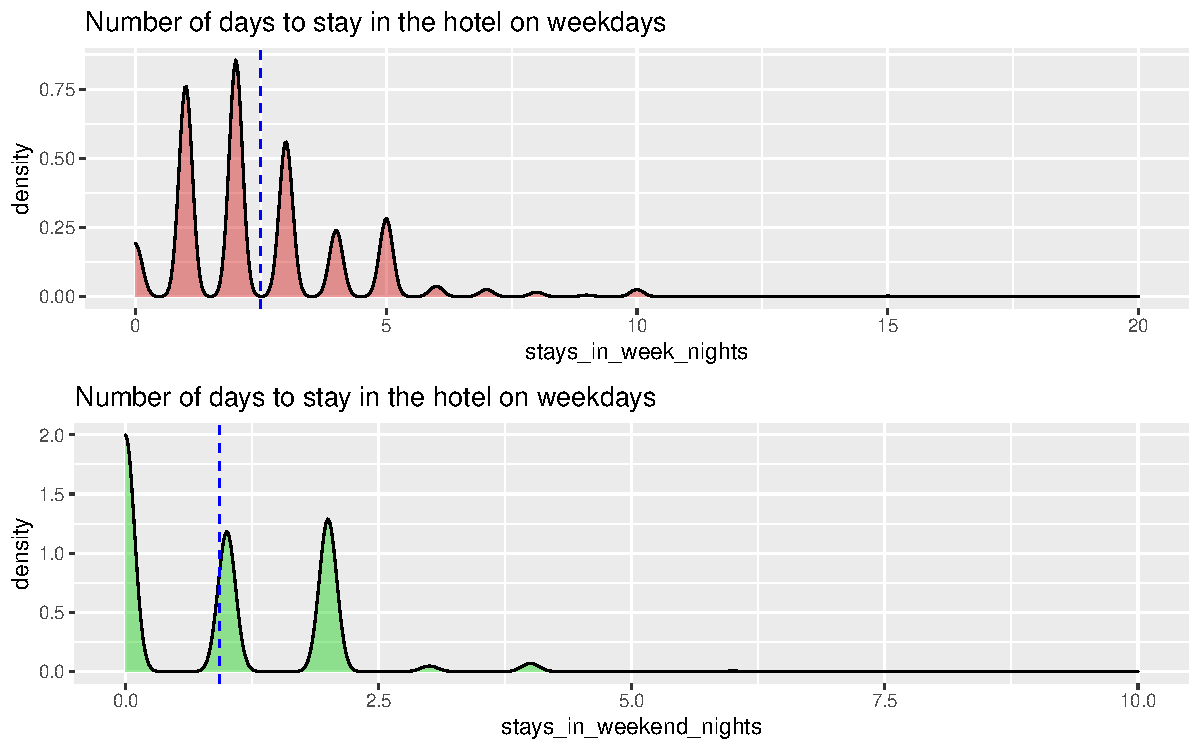
\includegraphics{tidy_files/figure-latex/unnamed-chunk-10-1.pdf}

What month is the peak of the hotel?
It can be seen from this chart that no matter what kind of hotel it is, April, August, and December are the peak periods for hotels.
For hotels, we recommend that more people be hired during this period to cope with the peak of passenger flow, so as not to reduce service quality, so as to bring a good experience to customers and increase the image of the hotel.
For customers, we recommend avoiding travel during these three months, and being able to travel off peaks and enjoy better hotel services.

\begin{Shaded}
\begin{Highlighting}[]
\NormalTok{month <-}\StringTok{ }\NormalTok{final }\OperatorTok
\StringTok{  }\NormalTok{dplyr}\OperatorTok{::}\KeywordTok{select}\NormalTok{(hotel,arrival_date_month,arrival_date_year) }\OperatorTok
\StringTok{  }\KeywordTok{filter}\NormalTok{(hotel}\OperatorTok{==}\StringTok{"Resort Hotel"}\NormalTok{)}
  
\NormalTok{mr<-}\KeywordTok{ggplot}\NormalTok{(month, }\KeywordTok{aes}\NormalTok{(}\DataTypeTok{x =}\NormalTok{arrival_date_month))}\OperatorTok{+}
\StringTok{  }\KeywordTok{geom_density}\NormalTok{(}\KeywordTok{aes}\NormalTok{(}\DataTypeTok{color=}\NormalTok{arrival_date_year),}\DataTypeTok{fill=}\StringTok{"greenyellow"}\NormalTok{,}\DataTypeTok{alpha=}\FloatTok{0.4}\NormalTok{)}\OperatorTok{+}
\StringTok{  }\KeywordTok{theme}\NormalTok{(}\DataTypeTok{axis.text.x =} \KeywordTok{element_text}\NormalTok{(}\DataTypeTok{angle =} \DecValTok{90}\NormalTok{))}\OperatorTok{+}
\StringTok{  }\KeywordTok{labs}\NormalTok{(}\DataTypeTok{title =} \StringTok{"the customer density plot by month in resort-hotel"}\NormalTok{)}\OperatorTok{+}
\StringTok{  }\KeywordTok{geom_vline}\NormalTok{(}\DataTypeTok{xintercept =} \KeywordTok{mean}\NormalTok{(month}\OperatorTok{$}\NormalTok{arrival_date_month),}\DataTypeTok{color=}\StringTok{"blue"}\NormalTok{, }\DataTypeTok{linetype=}\StringTok{"dashed"}\NormalTok{)}\OperatorTok{+}
\StringTok{  }\KeywordTok{facet_wrap}\NormalTok{(}\OperatorTok{~}\NormalTok{arrival_date_year)}



\NormalTok{month2 <-}\StringTok{ }\NormalTok{final }\OperatorTok
\StringTok{  }\NormalTok{dplyr}\OperatorTok{::}\KeywordTok{select}\NormalTok{(hotel,arrival_date_month,arrival_date_year) }\OperatorTok
\StringTok{  }\KeywordTok{filter}\NormalTok{(hotel}\OperatorTok{==}\StringTok{"City Hotel"}\NormalTok{)}
  
\NormalTok{mc<-}\KeywordTok{ggplot}\NormalTok{(month2, }\KeywordTok{aes}\NormalTok{(}\DataTypeTok{x =}\NormalTok{arrival_date_month))}\OperatorTok{+}
\StringTok{  }\KeywordTok{geom_density}\NormalTok{(}\KeywordTok{aes}\NormalTok{(}\DataTypeTok{color=}\NormalTok{arrival_date_year),}\DataTypeTok{fill=}\StringTok{"red3"}\NormalTok{,}\DataTypeTok{alpha=}\FloatTok{0.3}\NormalTok{)}\OperatorTok{+}
\StringTok{  }\KeywordTok{theme}\NormalTok{(}\DataTypeTok{axis.text.x =} \KeywordTok{element_text}\NormalTok{(}\DataTypeTok{angle =} \DecValTok{90}\NormalTok{))}\OperatorTok{+}
\StringTok{  }\KeywordTok{labs}\NormalTok{(}\DataTypeTok{title =} \StringTok{"the customer density plot by month in city-hotel"}\NormalTok{)}\OperatorTok{+}
\StringTok{  }\KeywordTok{geom_vline}\NormalTok{(}\DataTypeTok{xintercept =} \KeywordTok{mean}\NormalTok{(month}\OperatorTok{$}\NormalTok{arrival_date_month),}\DataTypeTok{color=}\StringTok{"blue"}\NormalTok{, }\DataTypeTok{linetype=}\StringTok{"dashed"}\NormalTok{)}\OperatorTok{+}
\StringTok{  }\KeywordTok{facet_wrap}\NormalTok{(}\OperatorTok{~}\NormalTok{arrival_date_year)}

\KeywordTok{grid.arrange}\NormalTok{(mr, mc, }\DataTypeTok{ncol =} \DecValTok{1}\NormalTok{)}
\end{Highlighting}
\end{Shaded}

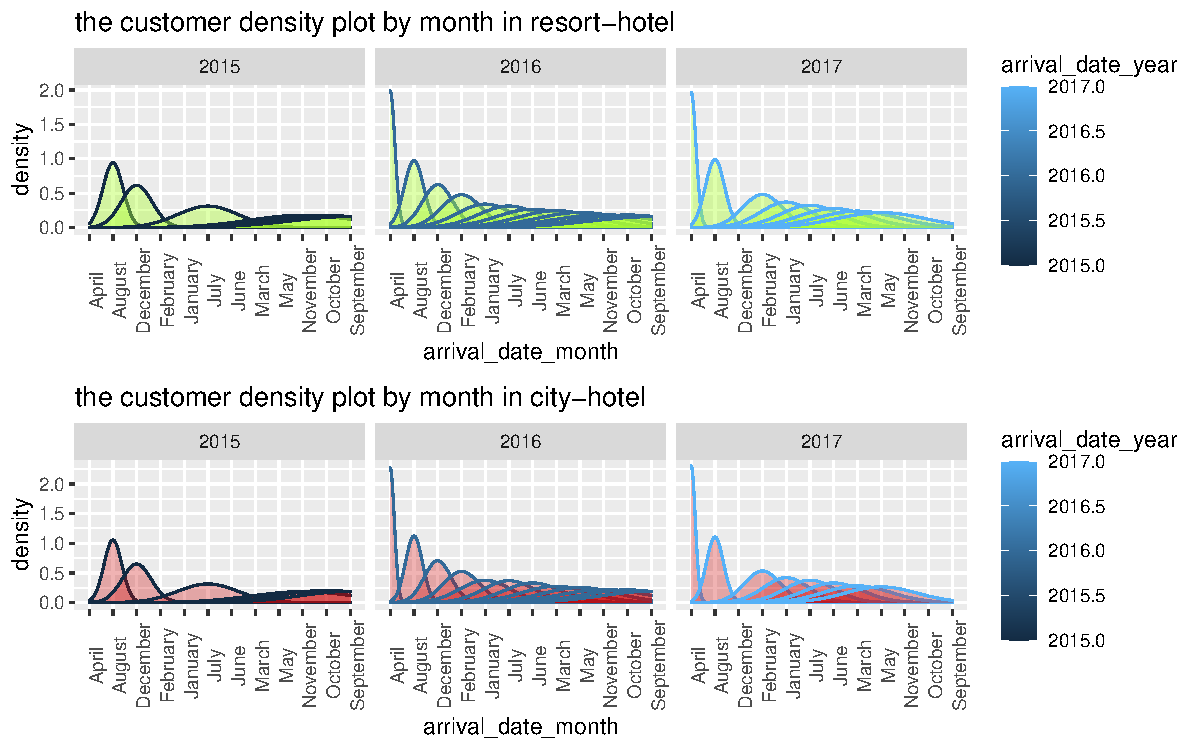
\includegraphics{tidy_files/figure-latex/unnamed-chunk-11-1.pdf}

\begin{center}\rule{0.5\linewidth}{0.5pt}\end{center}

1.Which day of the month is most common and which season (or month) has more customers in the whole year?

\begin{Shaded}
\begin{Highlighting}[]
\KeywordTok{library}\NormalTok{(plotly)}
\NormalTok{month_}\DecValTok{2016}\NormalTok{ <-}\StringTok{ }\NormalTok{final }\OperatorTok
\StringTok{  }\KeywordTok{filter}\NormalTok{(arrival_date_year }\OperatorTok{==}\StringTok{ }\DecValTok{2016}\NormalTok{) }\OperatorTok
\StringTok{  }\KeywordTok{group_by}\NormalTok{(arrival_date_day_of_month, arrival_date_month, hotel) }\OperatorTok
\StringTok{  }\KeywordTok{count}\NormalTok{(}\DataTypeTok{Count=}\KeywordTok{n}\NormalTok{())}

\NormalTok{g1 <-}\StringTok{ }\KeywordTok{ggplot}\NormalTok{(month_}\DecValTok{2016}\NormalTok{,}
       \KeywordTok{aes}\NormalTok{(}\DataTypeTok{x=}\NormalTok{arrival_date_day_of_month, }\DataTypeTok{y=}\NormalTok{Count, }\DataTypeTok{color=}\NormalTok{arrival_date_month)) }\OperatorTok{+}
\StringTok{  }\KeywordTok{xlab}\NormalTok{(}\StringTok{"Arrival day"}\NormalTok{) }\OperatorTok{+}
\StringTok{  }\KeywordTok{geom_col}\NormalTok{() }\OperatorTok{+}\StringTok{ }
\KeywordTok{theme}\NormalTok{(}\DataTypeTok{axis.text.x =} \KeywordTok{element_text}\NormalTok{()) }
  
\KeywordTok{ggplotly}\NormalTok{(g1)}
\end{Highlighting}
\end{Shaded}

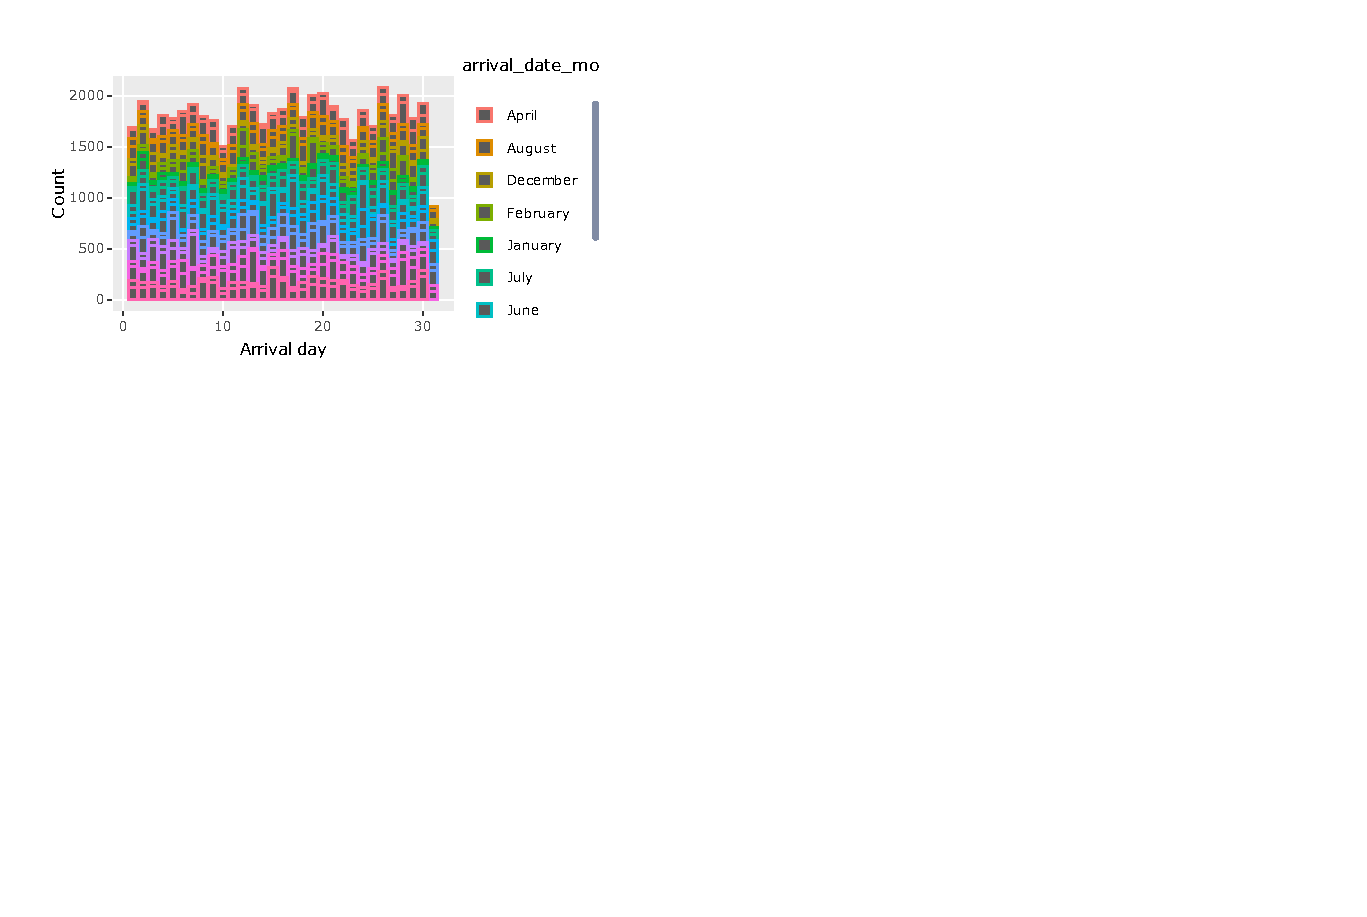
\includegraphics{tidy_files/figure-latex/unnamed-chunk-12-1.pdf}

\begin{Shaded}
\begin{Highlighting}[]
\NormalTok{month_}\DecValTok{2016}\OperatorTok{$}\NormalTok{arrival_date_month <-}\StringTok{ }\KeywordTok{factor}\NormalTok{ (month_}\DecValTok{2016}\OperatorTok{$}\NormalTok{arrival_date_month,}
                     \DataTypeTok{levels =} \KeywordTok{c}\NormalTok{(}\StringTok{"January"}\NormalTok{, }\StringTok{"February"}\NormalTok{, }\StringTok{"March"}\NormalTok{, }\StringTok{"April"}\NormalTok{, }\StringTok{"May"}\NormalTok{, }\StringTok{"June"}\NormalTok{, }\StringTok{"July"}\NormalTok{, }\StringTok{"August"}\NormalTok{, }\StringTok{"September"}\NormalTok{, }\StringTok{"October"}\NormalTok{, }\StringTok{"November"}\NormalTok{, }\StringTok{"December"}\NormalTok{))}

\NormalTok{month_book <-}\StringTok{ }\KeywordTok{ggplot}\NormalTok{(month_}\DecValTok{2016}\NormalTok{,}
       \KeywordTok{aes}\NormalTok{(}\DataTypeTok{x=}\NormalTok{arrival_date_month, }\DataTypeTok{y=}\NormalTok{Count, }\DataTypeTok{fill=}\NormalTok{hotel)) }\OperatorTok{+}
\StringTok{  }\KeywordTok{geom_bar}\NormalTok{(}\DataTypeTok{stat =} \StringTok{"identity"}\NormalTok{, }
\DataTypeTok{position =} \StringTok{"stack"}\NormalTok{) }\OperatorTok{+}\StringTok{ }
\StringTok{  }\KeywordTok{xlab}\NormalTok{(}\StringTok{"Month"}\NormalTok{) }\OperatorTok{+}
\KeywordTok{theme}\NormalTok{(}\DataTypeTok{axis.text.x =} \KeywordTok{element_text}\NormalTok{(}\DataTypeTok{angle =} \DecValTok{90}\NormalTok{, }\DataTypeTok{vjust =} \FloatTok{0.5}\NormalTok{, }\DataTypeTok{hjust=}\DecValTok{1}\NormalTok{))}
\NormalTok{month_book}
\end{Highlighting}
\end{Shaded}

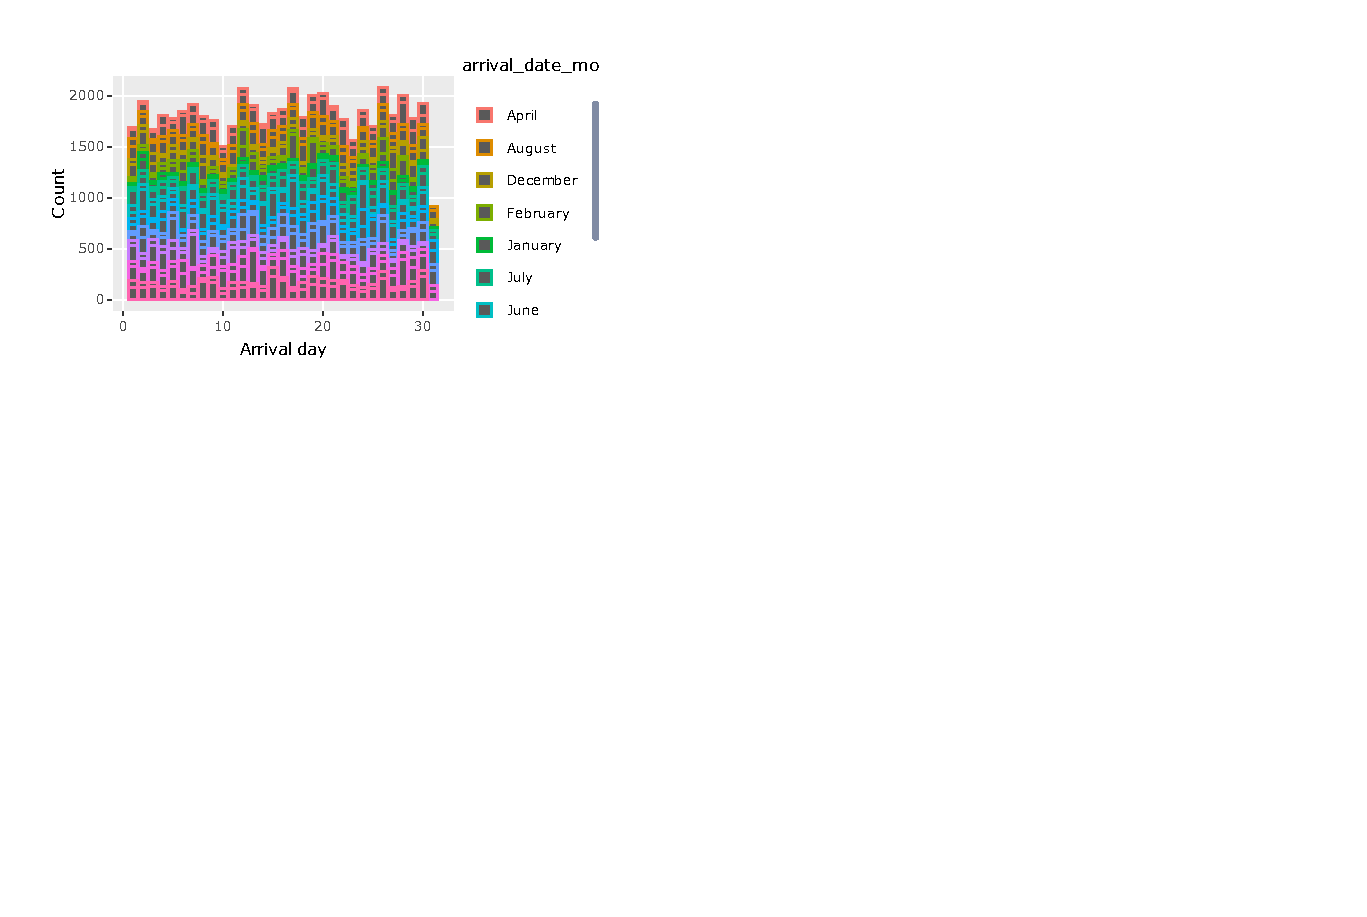
\includegraphics{tidy_files/figure-latex/unnamed-chunk-13-1.pdf}

2.Comparing the most reserved season by different hotel types with different countries.

\begin{Shaded}
\begin{Highlighting}[]
\KeywordTok{library}\NormalTok{(kableExtra)}
\KeywordTok{library}\NormalTok{(dplyr)}
\NormalTok{Top10Country <-}\StringTok{ }\NormalTok{final }\OperatorTok
\StringTok{  }\KeywordTok{count}\NormalTok{(Country, }\DataTypeTok{sort =}\NormalTok{ T) }\OperatorTok
\StringTok{  }\KeywordTok{head}\NormalTok{(}\DecValTok{10}\NormalTok{) }\OperatorTok
\StringTok{  }\KeywordTok{kable}\NormalTok{(}\DataTypeTok{caption =} \StringTok{"Top10 coutries reserved"}\NormalTok{)}
\NormalTok{Top10Country}
\end{Highlighting}
\end{Shaded}

\begin{table}

\caption{\label{tab:unnamed-chunk-14}Top10 coutries reserved}
\centering
\begin{tabular}[t]{l|r}
\hline
Country & n\\
\hline
Portugal & 48586\\
\hline
United Kingdom & 12129\\
\hline
France & 10415\\
\hline
Spain & 8568\\
\hline
Germany & 7287\\
\hline
Italy & 3766\\
\hline
Ireland & 3375\\
\hline
Belgium & 2342\\
\hline
Brazil & 2224\\
\hline
Netherlands & 2104\\
\hline
\end{tabular}
\end{table}

\begin{Shaded}
\begin{Highlighting}[]
\NormalTok{month_countries <-}\StringTok{ }\NormalTok{final }\OperatorTok
\StringTok{  }\KeywordTok{filter}\NormalTok{(arrival_date_year }\OperatorTok{==}\StringTok{ }\DecValTok{2016}\NormalTok{,}
\NormalTok{         Country }\OperatorTok\KeywordTok{c}\NormalTok{(}\StringTok{"Portugal"}\NormalTok{, }\StringTok{"United Kingdom"}\NormalTok{, }\StringTok{"Australia"}\NormalTok{, }\StringTok{"China"}\NormalTok{)) }\OperatorTok
\StringTok{  }\KeywordTok{group_by}\NormalTok{(arrival_date_month, hotel, Country) }\OperatorTok
\StringTok{  }\KeywordTok{count}\NormalTok{(}\DataTypeTok{Count=}\KeywordTok{n}\NormalTok{())}
\NormalTok{month_countries}\OperatorTok{$}\NormalTok{arrival_date_month <-}\StringTok{ }\KeywordTok{factor}\NormalTok{ (month_countries}\OperatorTok{$}\NormalTok{arrival_date_month,}
                     \DataTypeTok{levels =} \KeywordTok{c}\NormalTok{(}\StringTok{"January"}\NormalTok{, }\StringTok{"February"}\NormalTok{, }\StringTok{"March"}\NormalTok{, }\StringTok{"April"}\NormalTok{, }\StringTok{"May"}\NormalTok{, }\StringTok{"June"}\NormalTok{, }\StringTok{"July"}\NormalTok{, }\StringTok{"August"}\NormalTok{, }\StringTok{"September"}\NormalTok{, }\StringTok{"October"}\NormalTok{, }\StringTok{"November"}\NormalTok{, }\StringTok{"December"}\NormalTok{))}

\NormalTok{month_country <-}\StringTok{ }\KeywordTok{ggplot}\NormalTok{(month_countries,}
       \KeywordTok{aes}\NormalTok{(}\DataTypeTok{x=}\NormalTok{arrival_date_month, }\DataTypeTok{y=}\NormalTok{Count, }\DataTypeTok{fill=}\NormalTok{hotel)) }\OperatorTok{+}
\StringTok{  }\KeywordTok{geom_bar}\NormalTok{(}\DataTypeTok{stat =} \StringTok{"identity"}\NormalTok{, }
\DataTypeTok{position =} \StringTok{"stack"}\NormalTok{) }\OperatorTok{+}\StringTok{ }
\StringTok{  }\KeywordTok{xlab}\NormalTok{(}\StringTok{"Month"}\NormalTok{) }\OperatorTok{+}
\StringTok{  }\KeywordTok{facet_wrap}\NormalTok{(}\OperatorTok{~}\NormalTok{Country, }\DataTypeTok{scales =} \StringTok{"free_y"}\NormalTok{) }\OperatorTok{+}
\KeywordTok{theme}\NormalTok{(}\DataTypeTok{axis.text.x =} \KeywordTok{element_text}\NormalTok{(}\DataTypeTok{angle =} \DecValTok{90}\NormalTok{, }\DataTypeTok{vjust =} \FloatTok{0.5}\NormalTok{, }\DataTypeTok{hjust=}\DecValTok{1}\NormalTok{))}
\end{Highlighting}
\end{Shaded}

\begin{center}\rule{0.5\linewidth}{0.5pt}\end{center}

\hypertarget{q8which-countrys-people-most-like-to-repeat-to-reserve-these-hotels}{%
\subsection{Q8:Which country's people most like to repeat to reserve these hotels?}\label{q8which-countrys-people-most-like-to-repeat-to-reserve-these-hotels}}

(it is a question about the customer/booking)

People can find which country's people most like to repeat to reserve the same hotel, City Hotel or Resort Hotel when they come to Portugal from the bar plots.

The bar plots show the top 10 rank about the proportion of repeated guests for Resort Hotel and City Hotel for 2015 to 2017. It is obvious that the proportion of Resort Hotel was much higher than that of City Hotel. The proportion of customers from Portugal ranked first for City Hotel but it just ranked sixth for Resort Hotel.

The main reason for that may have something to do with the location of this two hotels.The City Hotel is located in the center of the country and there are more hotels in that place, so there are more options for customers to pick one hotel they like.While the Resort Hotel is located in the suburb, and there are not many options for customers to choose different hotels.So the proportion of repeated customers are higher in the Resort Hotel.

\begin{Shaded}
\begin{Highlighting}[]
\NormalTok{a <-}\StringTok{ }\NormalTok{final}\OperatorTok
\StringTok{  }\KeywordTok{select}\NormalTok{(hotel,Country,is_repeated_guest)}\OperatorTok
\StringTok{  }\KeywordTok{count}\NormalTok{(hotel,Country,is_repeated_guest)}\OperatorTok
\StringTok{  }\KeywordTok{pivot_wider}\NormalTok{(}\DataTypeTok{names_from=}\StringTok{"is_repeated_guest"}\NormalTok{,}\DataTypeTok{values_from=}\NormalTok{n)}\OperatorTok
\StringTok{  }\KeywordTok{rename}\NormalTok{(}\DataTypeTok{not_repeated_guest=}\StringTok{"0"}\NormalTok{,}\DataTypeTok{repeated_guest=}\StringTok{"1"}\NormalTok{)}\OperatorTok
\StringTok{  }\KeywordTok{filter}\NormalTok{(}\OperatorTok{!}\KeywordTok{is.na}\NormalTok{(repeated_guest))}\OperatorTok
\StringTok{  }\KeywordTok{mutate}\NormalTok{(}\DataTypeTok{prop=}\KeywordTok{round}\NormalTok{(repeated_guest}\OperatorTok{/}\NormalTok{(not_repeated_guest}\OperatorTok{+}\NormalTok{repeated_guest),}\DataTypeTok{digits=}\DecValTok{3}\NormalTok{))}\OperatorTok
\StringTok{  }\KeywordTok{arrange}\NormalTok{(}\KeywordTok{desc}\NormalTok{(prop))}\OperatorTok\StringTok{ }
\StringTok{  }\KeywordTok{ungroup}\NormalTok{()}\OperatorTok
\StringTok{  }\KeywordTok{slice_head}\NormalTok{(}\DataTypeTok{n =}\DecValTok{20}\NormalTok{)}

\NormalTok{prop_c <-}\StringTok{ }\NormalTok{a}\OperatorTok
\StringTok{  }\KeywordTok{filter}\NormalTok{(hotel}\OperatorTok{==}\StringTok{"City Hotel"}\NormalTok{)}\OperatorTok
\StringTok{  }\KeywordTok{ggplot}\NormalTok{(}\KeywordTok{aes}\NormalTok{(}\DataTypeTok{x=}\KeywordTok{reorder}\NormalTok{(Country,prop),}\DataTypeTok{y=}\NormalTok{prop))}\OperatorTok{+}
\StringTok{  }\KeywordTok{geom_col}\NormalTok{(}\DataTypeTok{show.legend =} \OtherTok{FALSE}\NormalTok{)}\OperatorTok{+}
\StringTok{  }\KeywordTok{coord_flip}\NormalTok{()}\OperatorTok{+}
\StringTok{  }\KeywordTok{theme_minimal}\NormalTok{()}\OperatorTok{+}
\StringTok{  }\KeywordTok{labs}\NormalTok{(}\DataTypeTok{title =} \StringTok{"Repeated guest proportion of City Hotel from July 2015 to August 2017"}\NormalTok{,}
       \DataTypeTok{x =} \StringTok{""}\NormalTok{,}
       \DataTypeTok{y=}\StringTok{"proportion"}\NormalTok{)}\OperatorTok{+}
\StringTok{  }\KeywordTok{theme}\NormalTok{(}\DataTypeTok{plot.title=}\KeywordTok{element_text}\NormalTok{(}\DataTypeTok{size=}\DecValTok{7}\NormalTok{))}\OperatorTok{+}
\StringTok{  }\KeywordTok{geom_text}\NormalTok{(}\KeywordTok{aes}\NormalTok{(}\DataTypeTok{label=}\NormalTok{prop),}\DataTypeTok{hjust =} \FloatTok{-0.008}\NormalTok{, }\DataTypeTok{size =} \DecValTok{2}\NormalTok{)}\OperatorTok{+}
\StringTok{  }\KeywordTok{scale_y_continuous}\NormalTok{(}\DataTypeTok{breaks=}\KeywordTok{seq}\NormalTok{(}\DecValTok{0}\NormalTok{,}\DecValTok{1}\NormalTok{,}\FloatTok{0.02}\NormalTok{))}


\NormalTok{prop_r <-}\StringTok{ }\NormalTok{a}\OperatorTok
\StringTok{  }\KeywordTok{filter}\NormalTok{(hotel}\OperatorTok{==}\StringTok{"Resort Hotel"}\NormalTok{)}\OperatorTok
\StringTok{  }\KeywordTok{ggplot}\NormalTok{(}\KeywordTok{aes}\NormalTok{(}\DataTypeTok{x=}\KeywordTok{reorder}\NormalTok{(Country,prop),}\DataTypeTok{y=}\NormalTok{prop))}\OperatorTok{+}
\StringTok{  }\KeywordTok{geom_col}\NormalTok{(}\DataTypeTok{show.legend =} \OtherTok{FALSE}\NormalTok{)}\OperatorTok{+}
\StringTok{  }\KeywordTok{coord_flip}\NormalTok{()}\OperatorTok{+}
\StringTok{  }\KeywordTok{theme_minimal}\NormalTok{()}\OperatorTok{+}
\StringTok{  }\KeywordTok{labs}\NormalTok{(}\DataTypeTok{title =} \StringTok{"Repeated guest proportion of Resort Hotel from July 2015 to August 2017"}\NormalTok{,}
       \DataTypeTok{x =} \StringTok{""}\NormalTok{,}
       \DataTypeTok{y=}\StringTok{"proportion"}\NormalTok{)}\OperatorTok{+}
\StringTok{  }\KeywordTok{theme}\NormalTok{(}\DataTypeTok{plot.title=}\KeywordTok{element_text}\NormalTok{(}\DataTypeTok{size=}\DecValTok{7}\NormalTok{))}\OperatorTok{+}
\StringTok{  }\KeywordTok{geom_text}\NormalTok{(}\KeywordTok{aes}\NormalTok{(}\DataTypeTok{label=}\NormalTok{prop),}\DataTypeTok{hjust =} \FloatTok{-0.008}\NormalTok{, }\DataTypeTok{size =} \DecValTok{2}\NormalTok{)}\OperatorTok{+}
\StringTok{  }\KeywordTok{scale_y_continuous}\NormalTok{(}\DataTypeTok{breaks=}\KeywordTok{seq}\NormalTok{(}\DecValTok{0}\NormalTok{,}\DecValTok{1}\NormalTok{,}\FloatTok{0.2}\NormalTok{))}

\KeywordTok{grid.arrange}\NormalTok{(prop_c,prop_r,}\DataTypeTok{ncol=}\DecValTok{2}\NormalTok{)}
\end{Highlighting}
\end{Shaded}

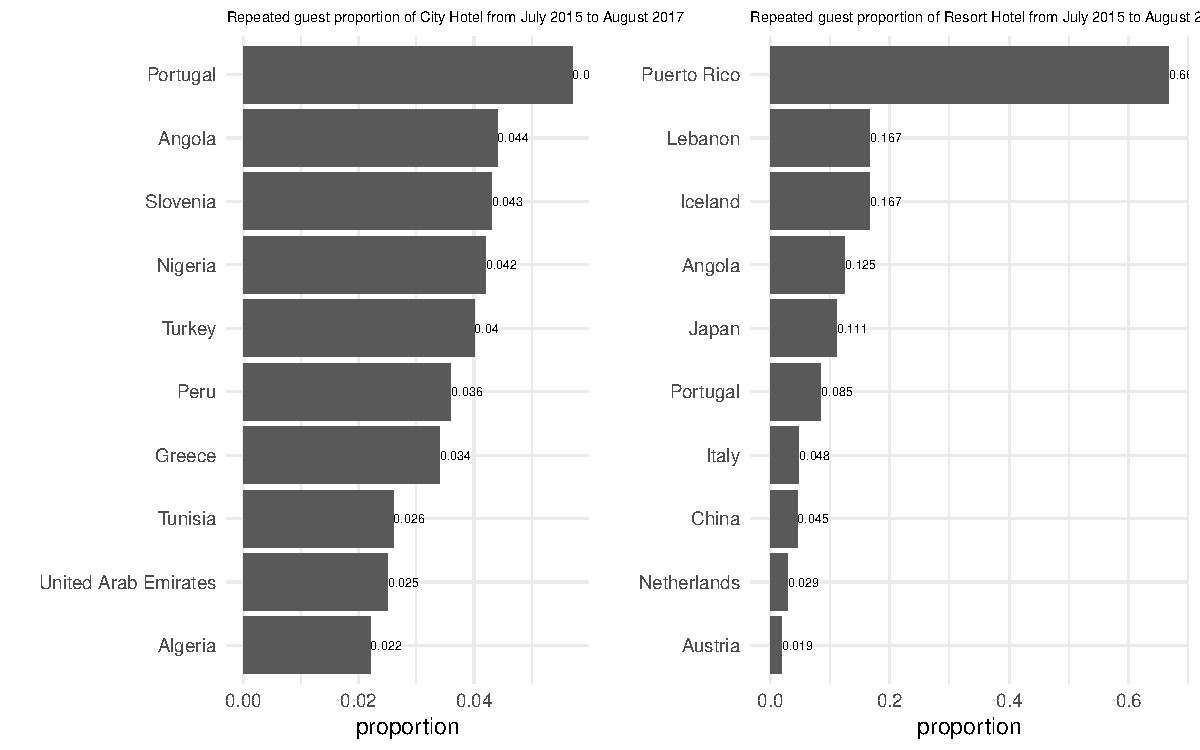
\includegraphics{tidy_files/figure-latex/Q8_1-1.pdf}

\hypertarget{q12how-close-to-the-arrival-date-is-the-booking-being-cancelled}{%
\subsection{Q12:How close to the arrival date is the booking being cancelled?}\label{q12how-close-to-the-arrival-date-is-the-booking-being-cancelled}}

(it is a question about the hotel/cancelled)

From the bar plots and density plots, people would clearly know that how close to the arrival data that customers have the most probability to cancel current booking.

It clearly shows that both of the two hotels have the similar distribution about the interval which represents the day between the original arrival day and the reservation cancelling day.

From the bar plots, people could find that to City Hotel, most of the interval is between 0 to 270 days while to Resort Hotel, that is between 0 to 150 days.

Both distributions in the density plots show a similar right skewed shape and they have the similar mean of the interval.

\begin{Shaded}
\begin{Highlighting}[]
\KeywordTok{library}\NormalTok{(lubridate)}
\NormalTok{plot_interval<-}\StringTok{ }\NormalTok{final}\OperatorTok
\StringTok{  }\KeywordTok{filter}\NormalTok{(is_canceled}\OperatorTok{==}\DecValTok{1}\NormalTok{)}\OperatorTok
\StringTok{  }\KeywordTok{select}\NormalTok{(hotel,is_canceled,reservation_status,reservation_status_date,arrival_time)}\OperatorTok
\StringTok{  }\KeywordTok{filter}\NormalTok{(reservation_status}\OperatorTok{==}\StringTok{"Canceled"}\NormalTok{)}\OperatorTok
\StringTok{  }\KeywordTok{mutate}\NormalTok{(}\DataTypeTok{reservation_status_date=}\KeywordTok{ymd}\NormalTok{(reservation_status_date),}
         \DataTypeTok{arrival_time=}\KeywordTok{ymd}\NormalTok{(arrival_time))}\OperatorTok
\StringTok{  }\KeywordTok{mutate}\NormalTok{(}\DataTypeTok{interval=}\NormalTok{arrival_time}\OperatorTok{-}\NormalTok{reservation_status_date)}

\NormalTok{interval <-}\StringTok{ }\NormalTok{plot_interval}\OperatorTok
\StringTok{  }\KeywordTok{ggplot}\NormalTok{(}\KeywordTok{aes}\NormalTok{(}\DataTypeTok{x=}\NormalTok{interval))}\OperatorTok{+}
\StringTok{  }\KeywordTok{geom_bar}\NormalTok{()}\OperatorTok{+}
\StringTok{  }\KeywordTok{scale_x_continuous}\NormalTok{(}\DataTypeTok{breaks=}\KeywordTok{seq}\NormalTok{(}\DecValTok{0}\NormalTok{,}\DecValTok{600}\NormalTok{,}\DecValTok{50}\NormalTok{))}\OperatorTok{+}
\StringTok{  }\KeywordTok{theme}\NormalTok{(}\DataTypeTok{axis.text.x=}\KeywordTok{element_text}\NormalTok{(}\DataTypeTok{angle=}\DecValTok{90}\NormalTok{))}\OperatorTok{+}
\StringTok{  }\KeywordTok{labs}\NormalTok{(}\DataTypeTok{x=}\StringTok{"interval(day)"}\NormalTok{)}\OperatorTok{+}
\StringTok{  }\KeywordTok{facet_wrap}\NormalTok{(}\OperatorTok{~}\NormalTok{hotel)}
\end{Highlighting}
\end{Shaded}

\begin{Shaded}
\begin{Highlighting}[]
\NormalTok{interval_c <-}\StringTok{ }\NormalTok{plot_interval}\OperatorTok
\StringTok{  }\KeywordTok{filter}\NormalTok{(hotel}\OperatorTok{==}\StringTok{"City Hotel"}\NormalTok{)}\OperatorTok
\StringTok{  }\KeywordTok{ggplot}\NormalTok{(}\KeywordTok{aes}\NormalTok{(}\DataTypeTok{x =}\NormalTok{ interval,}
             \DataTypeTok{y =}\NormalTok{ ..density..)) }\OperatorTok{+}
\StringTok{  }\KeywordTok{geom_density}\NormalTok{(}\DataTypeTok{fill =} \StringTok{"white"}\NormalTok{) }\OperatorTok{+}
\StringTok{  }\KeywordTok{geom_vline}\NormalTok{(}\DataTypeTok{xintercept =} \KeywordTok{mean}\NormalTok{(plot_interval}\OperatorTok{$}\NormalTok{interval),}
             \DataTypeTok{colour =} \StringTok{"red"}\NormalTok{)}\OperatorTok{+}
\StringTok{  }\KeywordTok{labs}\NormalTok{(}\DataTypeTok{x=}\StringTok{"interval(day)"}\NormalTok{)}

\NormalTok{interval_r <-}\StringTok{ }\NormalTok{plot_interval}\OperatorTok
\StringTok{  }\KeywordTok{filter}\NormalTok{(hotel}\OperatorTok{==}\StringTok{"Resort Hotel"}\NormalTok{)}\OperatorTok
\StringTok{  }\KeywordTok{ggplot}\NormalTok{(}\KeywordTok{aes}\NormalTok{(}\DataTypeTok{x =}\NormalTok{ interval,}
             \DataTypeTok{y =}\NormalTok{ ..density..)) }\OperatorTok{+}
\StringTok{  }\KeywordTok{geom_density}\NormalTok{(}\DataTypeTok{fill =} \StringTok{"white"}\NormalTok{) }\OperatorTok{+}
\StringTok{  }\KeywordTok{geom_vline}\NormalTok{(}\DataTypeTok{xintercept =} \KeywordTok{mean}\NormalTok{(plot_interval}\OperatorTok{$}\NormalTok{interval),}
             \DataTypeTok{colour =} \StringTok{"red"}\NormalTok{)}\OperatorTok{+}
\StringTok{  }\KeywordTok{labs}\NormalTok{(}\DataTypeTok{x=}\StringTok{"interval(day)"}\NormalTok{)}

\KeywordTok{grid.arrange}\NormalTok{(interval_c,interval_r,}\DataTypeTok{ncol=}\DecValTok{2}\NormalTok{)}
\end{Highlighting}
\end{Shaded}

\begin{verbatim}
## Don't know how to automatically pick scale for object of type difftime. Defaulting to continuous.
## Don't know how to automatically pick scale for object of type difftime. Defaulting to continuous.
\end{verbatim}

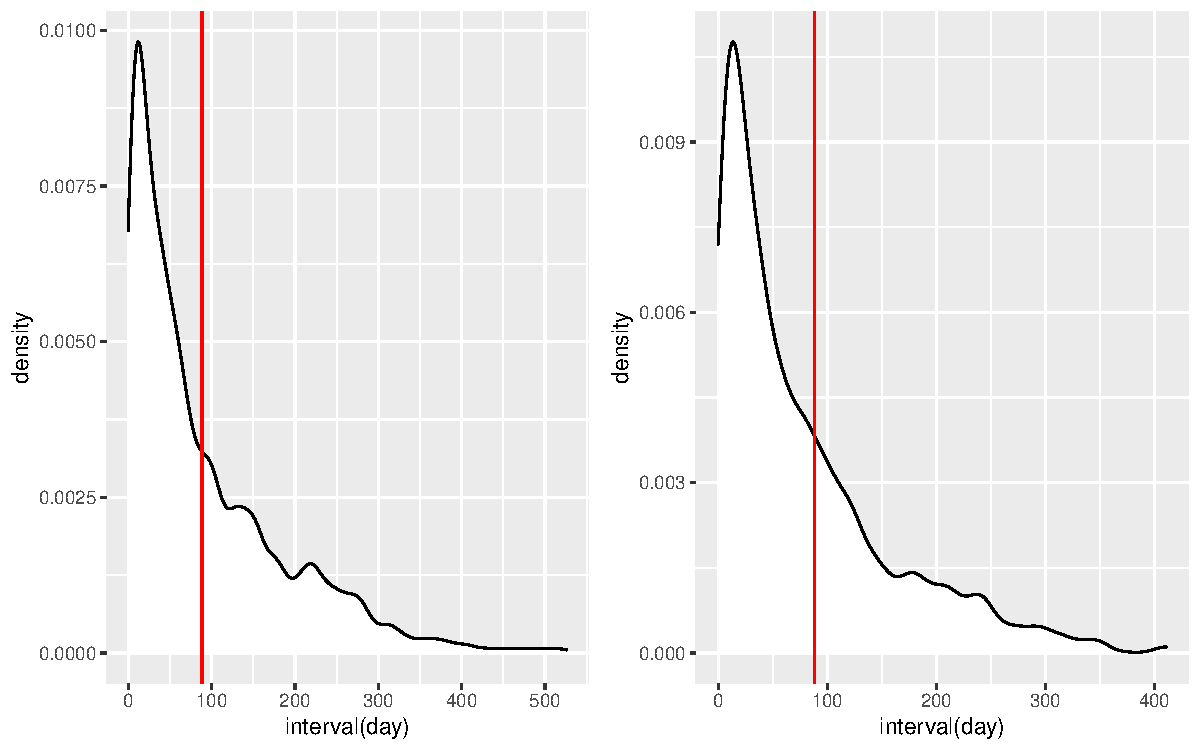
\includegraphics{tidy_files/figure-latex/Q12_2-1.pdf}

\begin{Shaded}
\begin{Highlighting}[]
\NormalTok{booking <-}\StringTok{ }\NormalTok{final }\OperatorTok\StringTok{ }\NormalTok{dplyr}\OperatorTok{::}\KeywordTok{select}\NormalTok{(lead_time,}
\NormalTok{                                 adr,}
\NormalTok{                                 is_canceled,}
\NormalTok{                                 reserved_room_type,}
\NormalTok{                                 assigned_room_type,}
\NormalTok{                                 arr_date_month, Country) }\OperatorTok
\StringTok{  }\KeywordTok{filter}\NormalTok{(is_canceled }\OperatorTok{==}\StringTok{ }\DecValTok{0}\NormalTok{) }
  \CommentTok{# mutate( change = ifelse(!reserved_room_type == assigned_room_type, 1,0),}
  \CommentTok{#         reserved_room_type = case_when(reserved_room_type == "A" ~ 0,}
  \CommentTok{#                                        reserved_room_type == "B" ~ 1,}
  \CommentTok{#                                        reserved_room_type == "C" ~ 2,}
  \CommentTok{#                                        reserved_room_type == "D" ~ 3,}
  \CommentTok{#                                        reserved_room_type == "E" ~ 4,}
  \CommentTok{#                                        reserved_room_type == "F" ~ 5,}
  \CommentTok{#                                        reserved_room_type == "G" ~ 6,}
  \CommentTok{#                                        reserved_room_type == "H" ~ 7,}
  \CommentTok{#                                        reserved_room_type == "I" ~ 8),}
  \CommentTok{#        assigned_room_type = case_when(assigned_room_type == "A" ~ 0,}
  \CommentTok{#                                        assigned_room_type== "B" ~ 1,}
  \CommentTok{#                                        assigned_room_type == "C" ~ 2,}
  \CommentTok{#                                       assigned_room_type == "D" ~ 3,}
  \CommentTok{#                                        assigned_room_type == "E" ~ 4,}
  \CommentTok{#                                        assigned_room_type == "F" ~ 5,}
  \CommentTok{#                                        assigned_room_type == "G" ~ 6,}
  \CommentTok{#                                       assigned_room_type == "H" ~ 7,}
  \CommentTok{#                                        assigned_room_type == "I" ~ 8)}
  \CommentTok{#         )}
\end{Highlighting}
\end{Shaded}

\begin{Shaded}
\begin{Highlighting}[]
\NormalTok{type <-}\StringTok{ }\NormalTok{booking }\OperatorTok\StringTok{ }
\StringTok{   }\KeywordTok{filter}\NormalTok{(}\OperatorTok{!}\NormalTok{reserved_room_type }\OperatorTok{==}\StringTok{ }\NormalTok{assigned_room_type) }\OperatorTok
\StringTok{  }\KeywordTok{group_by}\NormalTok{(lead_time, arr_date_month,reserved_room_type,assigned_room_type, Country) }\OperatorTok
\StringTok{  }\KeywordTok{count}\NormalTok{( }\DataTypeTok{name =} \StringTok{"Number"}\NormalTok{) }
\end{Highlighting}
\end{Shaded}

\begin{Shaded}
\begin{Highlighting}[]
\NormalTok{A <-}\StringTok{ }\NormalTok{type }\OperatorTok\StringTok{ }\KeywordTok{filter}\NormalTok{( arr_date_month }\OperatorTok{==}\StringTok{ "10"}\NormalTok{,}
\NormalTok{                      Country }\OperatorTok{==}\StringTok{ "United Kingdom"}\NormalTok{)}
=======
\NormalTok{vis\_tidy \textless{}{-}}\StringTok{ }\KeywordTok{vis\_miss}\NormalTok{(sec\_mute, }\DataTypeTok{warn\_large\_data =}\OtherTok{FALSE}\NormalTok{)}
\NormalTok{vis\_tidy}
\end{Highlighting}
\end{Shaded}

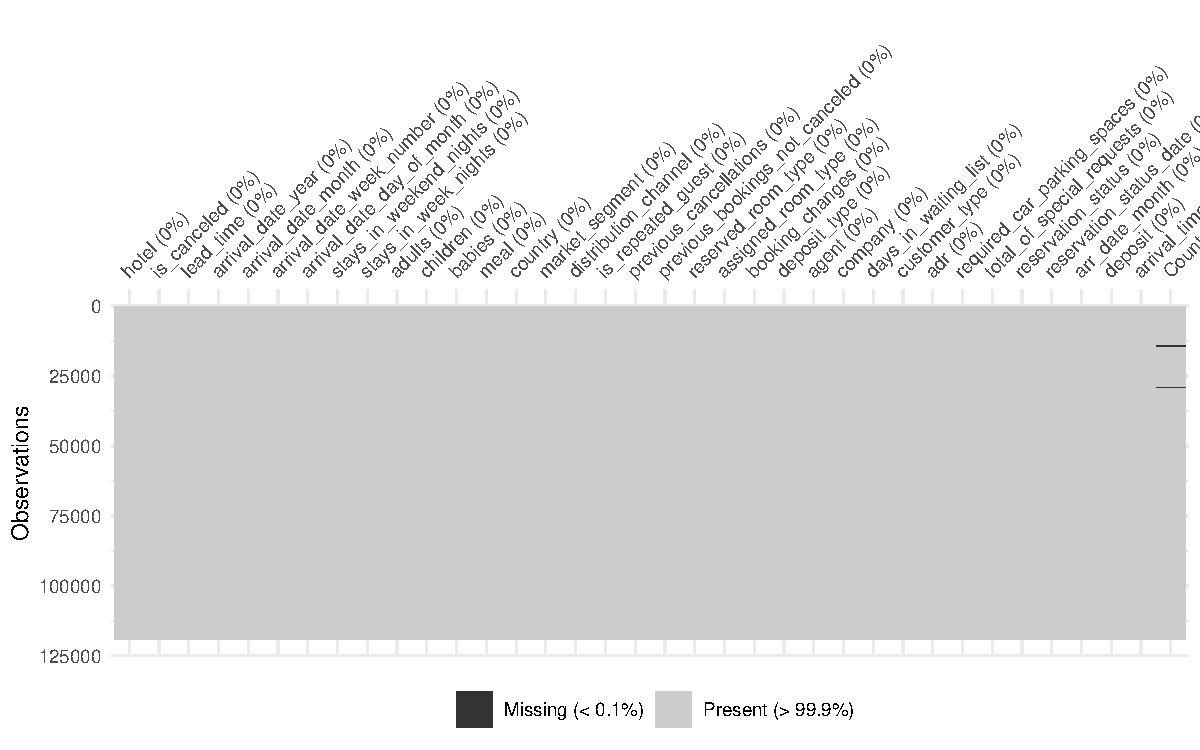
\includegraphics{tidy_files/figure-latex/sectidy-1.pdf}

\begin{Shaded}
\begin{Highlighting}[]
\NormalTok{sec\_mute \textless{}{-}}\StringTok{ }\NormalTok{sec\_mute  }\OperatorTok{\%\textgreater{}\%}\StringTok{ }\NormalTok{dplyr}\OperatorTok{::}\KeywordTok{select}\NormalTok{(}\OperatorTok{{-}}\NormalTok{market\_segment,}
                               \OperatorTok{{-}}\NormalTok{distribution\_channel,}
                               \OperatorTok{{-}}\NormalTok{deposit\_type,}
                               \OperatorTok{{-}}\NormalTok{agent,}
                               \OperatorTok{{-}}\NormalTok{company) }
>>>>>>> master
\end{Highlighting}
\end{Shaded}

\begin{Shaded}
\begin{Highlighting}[]
<<<<<<< HEAD
\KeywordTok{ggplot}\NormalTok{(type, }\KeywordTok{aes}\NormalTok{(}\DataTypeTok{x =} \KeywordTok{factor}\NormalTok{(arr_date_month), }\DataTypeTok{y =}\NormalTok{ lead_time, }\DataTypeTok{size =}\NormalTok{ Number)) }\OperatorTok{+}
\StringTok{       }\KeywordTok{geom_point}\NormalTok{(}\DataTypeTok{shape =}\DecValTok{21}\NormalTok{, }\DataTypeTok{colour =} \StringTok{"#95CDF7"}\NormalTok{, }\DataTypeTok{fill =} \StringTok{"#F8BBD0"}\NormalTok{) }\OperatorTok{+}\StringTok{    }
\StringTok{     }\KeywordTok{scale_x_discrete}\NormalTok{( }\DataTypeTok{name =} \StringTok{"Month"}\NormalTok{ ) }\OperatorTok{+}
\StringTok{     }\KeywordTok{scale_y_continuous}\NormalTok{()}
\end{Highlighting}
\end{Shaded}

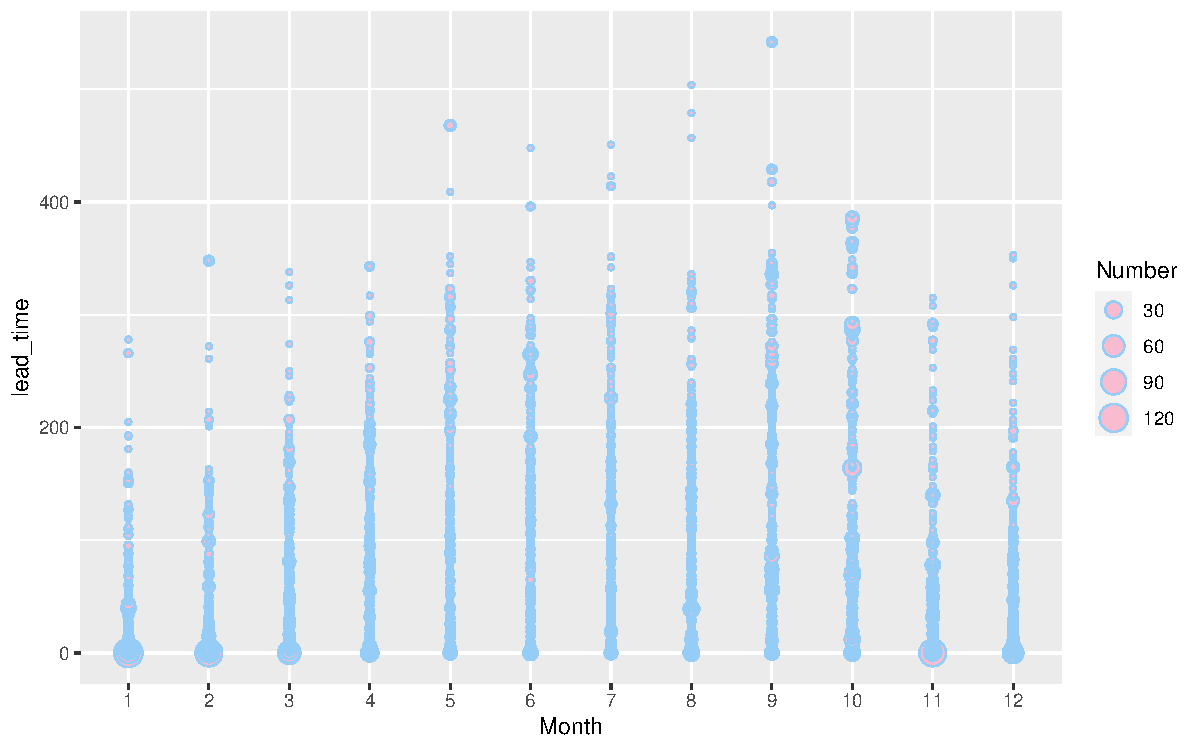
\includegraphics{tidy_files/figure-latex/leadtimeplot-1.pdf}

\begin{Shaded}
\begin{Highlighting}[]
\NormalTok{p <-}\StringTok{ }\KeywordTok{ggplot}\NormalTok{(A, }\KeywordTok{aes}\NormalTok{(}\DataTypeTok{x=}\NormalTok{ reserved_room_type , }\DataTypeTok{y =} \KeywordTok{log}\NormalTok{(Number}\OperatorTok{*}\DecValTok{2}\NormalTok{), }\DataTypeTok{fill =}\NormalTok{ assigned_room_type)) }\OperatorTok{+}
\StringTok{  }\KeywordTok{geom_bar}\NormalTok{(}\DataTypeTok{stat =} \StringTok{"identity"}\NormalTok{, }\DataTypeTok{alpha =} \FloatTok{0.7}\NormalTok{) }\OperatorTok{+}
\StringTok{ }\KeywordTok{theme_minimal}\NormalTok{() }\OperatorTok{+}
\StringTok{  }\KeywordTok{coord_polar}\NormalTok{() }
  

\NormalTok{p  }
\end{Highlighting}
\end{Shaded}

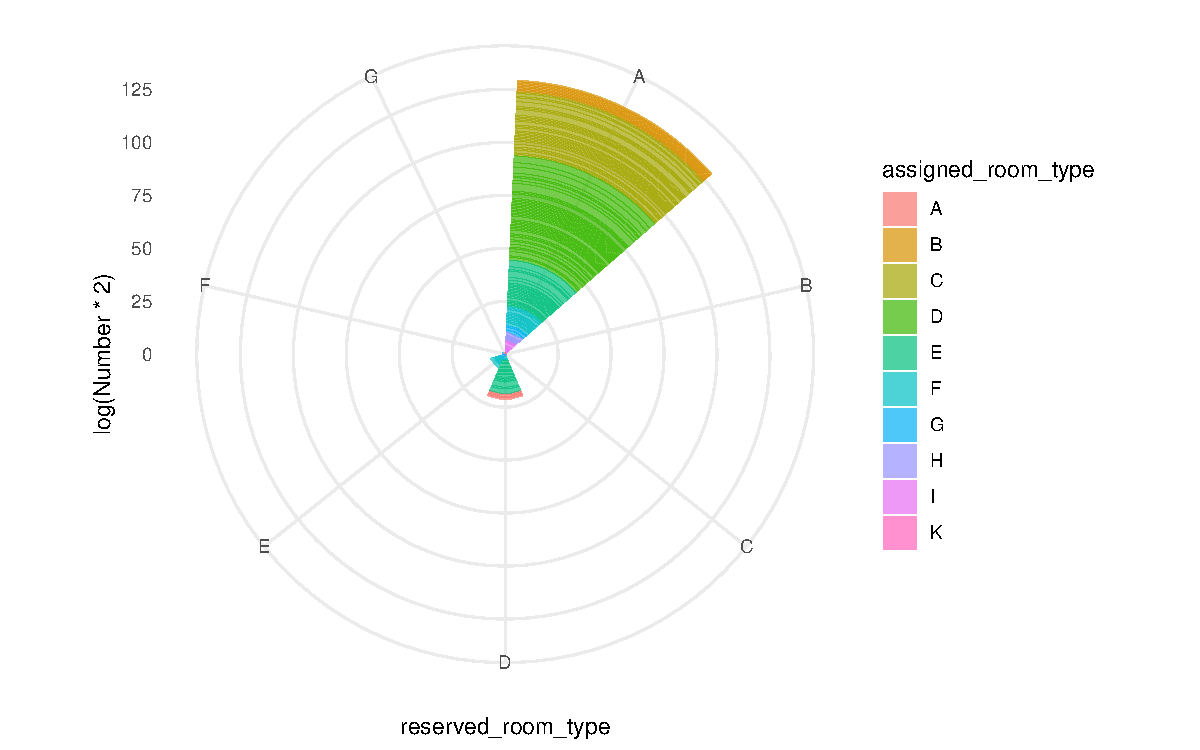
\includegraphics{tidy_files/figure-latex/coordplot-1.pdf}

\begin{Shaded}
\begin{Highlighting}[]
\NormalTok{interval_c <-}\StringTok{ }\NormalTok{plot_interval}\OperatorTok
\StringTok{  }\KeywordTok{filter}\NormalTok{(hotel}\OperatorTok{==}\StringTok{"City Hotel"}\NormalTok{)}

\NormalTok{interval_r <-}\StringTok{ }\NormalTok{plot_interval}\OperatorTok
\StringTok{  }\KeywordTok{filter}\NormalTok{(hotel}\OperatorTok{==}\StringTok{"Resort Hotel"}\NormalTok{)}

\NormalTok{plot_combined <-}\StringTok{ }\NormalTok{plot_interval}\OperatorTok
\StringTok{  }\KeywordTok{ggplot}\NormalTok{(}\KeywordTok{aes}\NormalTok{(interval,}\DataTypeTok{fill=}\KeywordTok{as.factor}\NormalTok{(hotel)))}\OperatorTok{+}
\StringTok{  }\KeywordTok{geom_density}\NormalTok{(}\DataTypeTok{alpha=}\FloatTok{0.3}\NormalTok{)}\OperatorTok{+}
\StringTok{  }\KeywordTok{geom_vline}\NormalTok{(}\DataTypeTok{xintercept =} \KeywordTok{mean}\NormalTok{(interval_c}\OperatorTok{$}\NormalTok{interval),}
             \DataTypeTok{colour =} \StringTok{"red"}\NormalTok{)}\OperatorTok{+}
\StringTok{  }\KeywordTok{geom_vline}\NormalTok{(}\DataTypeTok{xintercept =} \KeywordTok{mean}\NormalTok{(interval_r}\OperatorTok{$}\NormalTok{interval),}
             \DataTypeTok{colour =} \StringTok{"blue"}\NormalTok{)}\OperatorTok{+}
\StringTok{  }\KeywordTok{labs}\NormalTok{(}\DataTypeTok{x=}\StringTok{"interval(day)"}\NormalTok{)}

\NormalTok{plot_combined}
\end{Highlighting}
\end{Shaded}

\begin{verbatim}
## Don't know how to automatically pick scale for object of type difftime. Defaulting to continuous.
\end{verbatim}

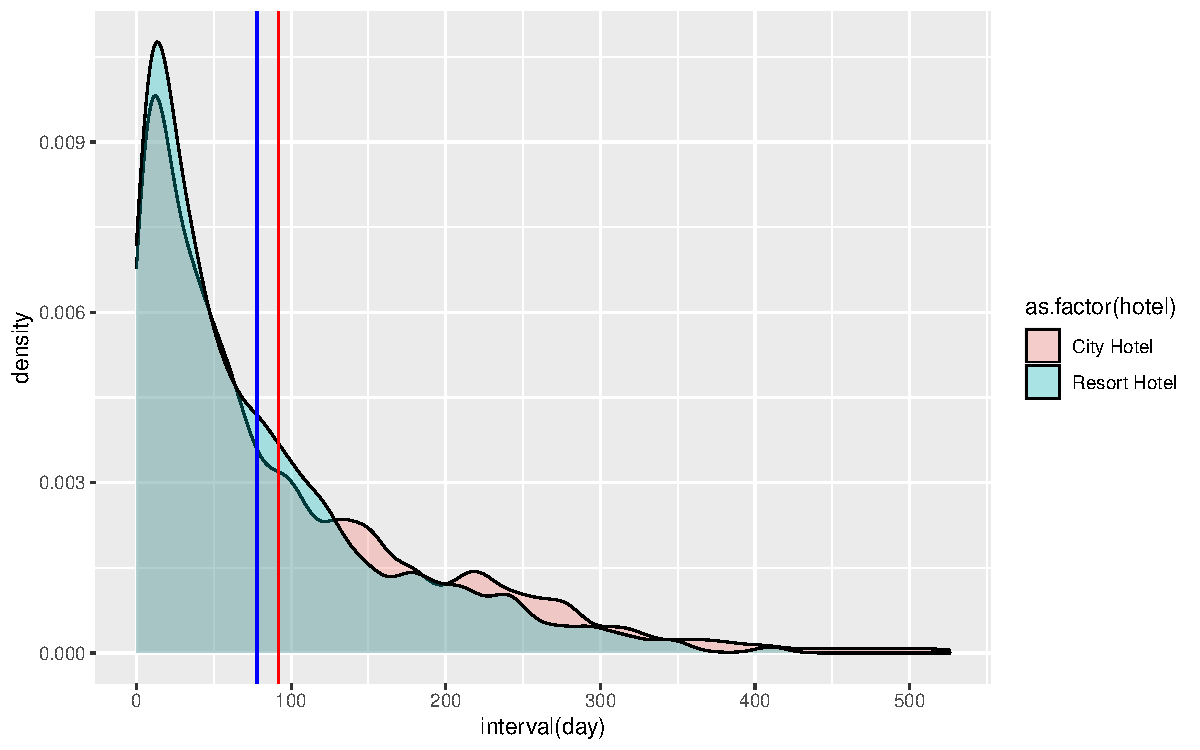
\includegraphics{tidy_files/figure-latex/intervaldensity-1.pdf}
=======
\NormalTok{final \textless{}{-}}\StringTok{ }\KeywordTok{na.omit}\NormalTok{(sec\_mute)  }\CommentTok{\# Delete the missing country observations}
\end{Highlighting}
\end{Shaded}

>>>>>>> master

\printbibliography

\end{document}
<<<<<<< HEAD

=======
>>>>>>> master
